% =====================================================================
%  Manual de funcionamiento y uso de la MPA (Módulo de Posición Angular)
%  Sistemas de Control en Tiempo Continuo - Ingeniería Mecatrónica, EIA
%  Prof. Sergio Andrés Castaño Giraldo
%  Compila con pdfLaTeX (Overleaf). Carpeta figs/ junto a este archivo.
% =====================================================================
\documentclass[11pt,letterpaper]{article}

\newcommand{\curso}{Sistemas de Control en Tiempo Continuo}
\newcommand{\programa}{Ingeniería Mecatrónica}
\newcommand{\semestre}{revisión 2026-2}

\usepackage[T1]{fontenc}
\usepackage[utf8]{inputenc}
\usepackage{babel}
\babelprovide[import,main]{spanish}
\usepackage{courier}
\usepackage{helvet}
\renewcommand{\familydefault}{\sfdefault}
\usepackage[margin=2.1cm,top=2.6cm,headheight=34pt,headsep=12pt]{geometry}
\usepackage{amsmath,amssymb}
\usepackage[per-mode=symbol,output-decimal-marker={.}]{siunitx}
\usepackage{graphicx}
\usepackage[table]{xcolor}
\usepackage{tikz}
\usetikzlibrary{positioning,arrows.meta,calc,shapes.misc,shapes.geometric,fit,backgrounds,decorations.pathreplacing,patterns}
\usepackage[american]{circuitikz}
\usepackage{pgfplots}
\pgfplotsset{compat=1.18}
\usepackage[most]{tcolorbox}
\usepackage{enumitem}
\usepackage{booktabs,tabularx,array,multirow}
\usepackage{fancyhdr}
\usepackage{caption}
\usepackage{float}
\usepackage{needspace}
\usepackage{listings}
\usepackage{titlesec}
\usepackage{tocloft}
\usepackage[hidelinks]{hyperref}

% ---------------------------------------------------------------------
\definecolor{azulEIA}{HTML}{003A70}
\definecolor{azulClaro}{HTML}{E8EEF6}
\definecolor{ambar}{HTML}{B45309}
\definecolor{ambarClaro}{HTML}{FDF3E1}
\definecolor{rojoAviso}{HTML}{B42318}
\definecolor{rojoClaro}{HTML}{FDECEC}
\definecolor{verdeOK}{HTML}{0F7B3F}
\definecolor{verdeClaro}{HTML}{E7F4EC}
\definecolor{gris}{HTML}{6B7280}
\definecolor{codigoFondo}{HTML}{F6F7F9}

\captionsetup{font=small,labelfont={bf,color=azulEIA}}
\setlist{itemsep=2pt,topsep=3pt}
\setlength{\parindent}{0pt}
\setlength{\parskip}{5pt}

\titleformat{\section}{\needspace{11\baselineskip}\color{azulEIA}\large\bfseries}{\thesection.}{0.5em}{}[{\color{azulEIA}\vspace{-4pt}\rule{\linewidth}{0.8pt}}]
\titleformat{\subsection}{\needspace{5\baselineskip}\color{azulEIA}\normalsize\bfseries}{\thesubsection}{0.5em}{}
\titlespacing*{\section}{0pt}{14pt}{6pt}
\titlespacing*{\subsection}{0pt}{10pt}{3pt}
\renewcommand{\cftsecfont}{\bfseries\color{azulEIA}}
\renewcommand{\cftsecpagefont}{\bfseries\color{azulEIA}}
\setlength{\cftbeforesecskip}{3pt}
\setcounter{tocdepth}{1}

\newtcolorbox{nota}[1][Nota]{enhanced,breakable,colback=azulClaro,colframe=azulEIA,
  boxrule=0.6pt,left=6pt,right=6pt,top=4pt,bottom=4pt,
  fonttitle=\bfseries\small,title={#1},sharp corners=south}
\newtcolorbox{cuidado}[1][Cuidado]{enhanced,breakable,colback=ambarClaro,colframe=ambar,
  boxrule=0.6pt,left=6pt,right=6pt,top=4pt,bottom=4pt,
  fonttitle=\bfseries\small,title={#1},sharp corners=south}
\newtcolorbox{peligro}[1][Seguridad]{enhanced,breakable,colback=rojoClaro,colframe=rojoAviso,
  boxrule=0.6pt,left=6pt,right=6pt,top=4pt,bottom=4pt,
  fonttitle=\bfseries\small,title={#1},sharp corners=south}
\newtcolorbox{pasos}[1][Pasos]{enhanced,breakable,colback=verdeClaro,colframe=verdeOK,
  boxrule=0.6pt,left=6pt,right=6pt,top=4pt,bottom=4pt,
  fonttitle=\bfseries\small,title={#1},sharp corners=south}

\newcommand{\blq}[1]{\textsf{\textbf{#1}}}                 % bloque de Simulink
\newcommand{\sen}[1]{\texttt{\detokenize{#1}}}             % señal / variable
\newcommand{\ficha}{\textcolor{verdeOK}{\textbf{[ficha]}}}  % dato que va a la ficha

\lstdefinestyle{matlab}{language=Matlab,basicstyle=\ttfamily\footnotesize,
  backgroundcolor=\color{codigoFondo},frame=single,rulecolor=\color{gray!40},
  keywordstyle=\color{azulEIA}\bfseries,commentstyle=\color{verdeOK},
  stringstyle=\color{ambar},showstringspaces=false,breaklines=true,
  columns=fullflexible,keepspaces=true,captionpos=t,
  xleftmargin=4pt,xrightmargin=4pt,aboveskip=6pt,belowskip=4pt}
\lstset{style=matlab}
\renewcommand{\lstlistingname}{Código}

\pagestyle{fancy}\fancyhf{}
\fancyhead[L]{\small\color{azulEIA}\textbf{\curso}\\\footnotesize \programa\ $\cdot$ Universidad EIA $\cdot$ \semestre}
\fancyhead[R]{\small\color{azulEIA}Manual de la MPA}
\renewcommand{\headrule}{{\color{azulEIA}\hrule height 0.8pt}}
\fancyfoot[L]{\footnotesize Prof. Sergio Andrés Castaño Giraldo}
\fancyfoot[R]{\footnotesize \thepage}

\tikzset{
  >=Stealth,
  blk/.style={draw=azulEIA,thick,fill=azulClaro,rounded corners=2pt,minimum height=8mm,minimum width=14mm,align=center,font=\footnotesize},
  blkw/.style={draw=azulEIA,thick,fill=white,rounded corners=2pt,minimum height=8mm,minimum width=14mm,align=center,font=\footnotesize},
  blka/.style={draw=ambar,thick,fill=ambarClaro,rounded corners=2pt,minimum height=8mm,minimum width=14mm,align=center,font=\footnotesize},
  blkv/.style={draw=verdeOK,thick,fill=verdeClaro,rounded corners=2pt,minimum height=8mm,minimum width=14mm,align=center,font=\footnotesize},
  sum/.style={draw=azulEIA,thick,circle,fill=white,inner sep=0pt,minimum size=4.5mm,font=\scriptsize},
  lab/.style={font=\scriptsize,color=gris},
  sig/.style={font=\scriptsize},
}

% =====================================================================
\begin{document}
\thispagestyle{empty}

\begin{tcolorbox}[enhanced,colback=azulEIA,colframe=azulEIA,sharp corners,left=10pt,right=10pt,top=8pt,bottom=8pt]
\begin{minipage}[c]{0.20\linewidth}
  
\includegraphics[width=\linewidth]{figs/logo_eia_blanco.png}
\end{minipage}\hfill
\begin{minipage}[c]{0.76\linewidth}\color{white}
  {\small \curso\ $\cdot$ \programa\ $\cdot$ \semestre}\\[3pt]
  \raggedright{\LARGE\bfseries Manual de funcionamiento y uso de la MPA}\\[3pt]
  {\large Módulo de posición angular: conexión, enlace con Simulink, calibración, ensayos e identificación de un modelo en espacio de estados}
\end{minipage}
\end{tcolorbox}

\begin{tcolorbox}[enhanced,colback=white,colframe=azulEIA,boxrule=0.8pt,sharp corners,left=8pt,right=8pt,top=5pt,bottom=5pt]
\begin{tabularx}{\linewidth}{@{}>{\bfseries\color{azulEIA}}l X@{}}
Planta & Lámina de acrílico que cuelga de un eje y que el chorro de una hélice levanta. Entrada: mando $u$ [\%]. Salida: ángulo $\theta$ [°], medido con un potenciómetro.\\
Enlace & Firmware propio en el Arduino y bloques seriales en Simulink. El Arduino marca el reloj (50~Hz), aplica el mando al ESC con rampa y tope, y vigila la comunicación.\\
Software & MATLAB y Simulink con el \emph{Instrument Control Toolbox} (bloques \emph{Serial}). Arduino IDE para cargar el firmware una vez.\\
Qué sale de aquí & La \textbf{ficha de su módulo} (calibración, límites del mando, mapa estático) y un \textbf{modelo lineal} $\dot x = Ax+Bu$, $y=Cx$ alrededor de un punto de operación, con estados físicos (ángulo y velocidad angular).\\
Qué no está aquí & El diseño del controlador y del observador: eso es el Reto In-Situ 3. Este manual deja la planta, el modelo y la interfaz de lazo cerrado listos para él.
\end{tabularx}
\end{tcolorbox}

\vspace{2pt}
{\small\tableofcontents}

% =====================================================================
\section{Antes de empezar}

El laboratorio tiene seis MPA. Todas son el mismo diseño, pero no son idénticas: han sido reparadas en momentos distintos, los potenciómetros y los ESC no son todos iguales y cada lámina tiene su propio rozamiento. Por eso \textbf{nada de lo que se mide aquí se copia de otra unidad}. Cada módulo tiene una \textbf{ficha} (anexo~\ref{sec:ficha}) donde quedan sus datos; si ya está llena, la primera tarea es comprobar tres de sus valores. En el texto, la marca \ficha\ indica un dato que va a la ficha.

\begin{figure}[H]\centering
\resizebox{\linewidth}{!}{%
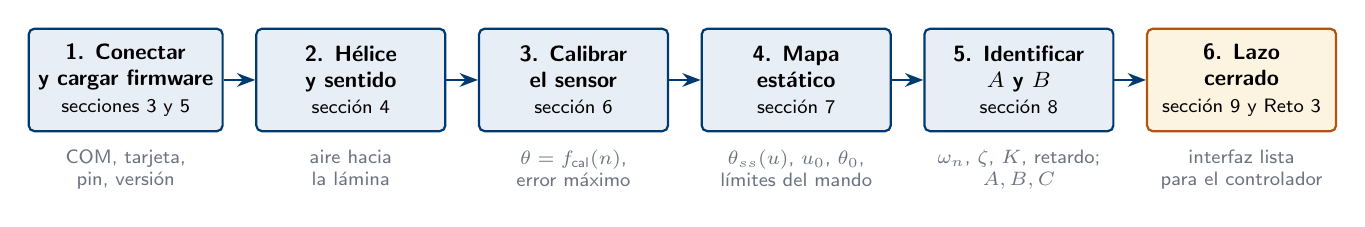
\begin{tikzpicture}[node distance=4mm]
  \node[blk,minimum width=24mm,minimum height=13mm] (e1) {\textbf{1. Conectar}\\\textbf{y cargar firmware}\\\scriptsize secciones 3 y 5};
  \node[blk,minimum width=24mm,minimum height=13mm,right=of e1] (e2) {\textbf{2. Hélice}\\\textbf{y sentido}\\\scriptsize sección 4};
  \node[blk,minimum width=24mm,minimum height=13mm,right=of e2] (e3) {\textbf{3. Calibrar}\\\textbf{el sensor}\\\scriptsize sección 6};
  \node[blk,minimum width=24mm,minimum height=13mm,right=of e3] (e4) {\textbf{4. Mapa}\\\textbf{estático}\\\scriptsize sección 7};
  \node[blk,minimum width=24mm,minimum height=13mm,right=of e4] (e5) {\textbf{5. Identificar}\\\textbf{$A$ y $B$}\\\scriptsize sección 8};
  \node[blka,minimum width=24mm,minimum height=13mm,right=of e5] (e6) {\textbf{6. Lazo}\\\textbf{cerrado}\\\scriptsize sección 9 y Reto 3};
  \foreach \a/\b in {e1/e2,e2/e3,e3/e4,e4/e5,e5/e6} \draw[->,thick,azulEIA] (\a) -- (\b);
  \node[lab,below=1mm of e1,align=center] {COM, tarjeta,\\pin, versión};
  \node[lab,below=1mm of e2,align=center] {aire hacia\\la lámina};
  \node[lab,below=1mm of e3,align=center] {$\theta=f_\text{cal}(n)$,\\error máximo};
  \node[lab,below=1mm of e4,align=center] {$\theta_{ss}(u)$, $u_0$, $\theta_0$,\\límites del mando};
  \node[lab,below=1mm of e5,align=center] {$\omega_n$, $\zeta$, $K$, retardo;\\$A,B,C$};
  \node[lab,below=1mm of e6,align=center] {interfaz lista\\para el controlador};
\end{tikzpicture}}
\caption{Ruta de trabajo. Debajo de cada etapa, lo que queda en la ficha.}\label{fig:ruta}
\end{figure}

\begin{nota}[Reglas de trabajo]
\begin{itemize}[leftmargin=12pt]
  \item \textbf{Un archivo de Simulink por etapa}, guardado con el número del módulo (\texttt{MPA\_XX\_ensayos.slx}, \texttt{MPA\_XX\_lazo.slx}). No reutilicen el de otra pareja: arrastra su calibración.
  \item \textbf{Todo dato se guarda con su contexto}: módulo, fecha, punto de operación y amplitud del ensayo.
  \item \textbf{Nunca abran un modelo de la MPA en Connected IO ni en Run on board}: Simulink reemplazaría el firmware del Arduino por el suyo y habría que volver a cargarlo (sección~\ref{sec:firmware}).
\end{itemize}
\end{nota}

% =====================================================================
\section{La planta y por qué se comporta como un péndulo}

\begin{figure}[H]\centering
\begin{minipage}[t]{0.32\linewidth}\centering
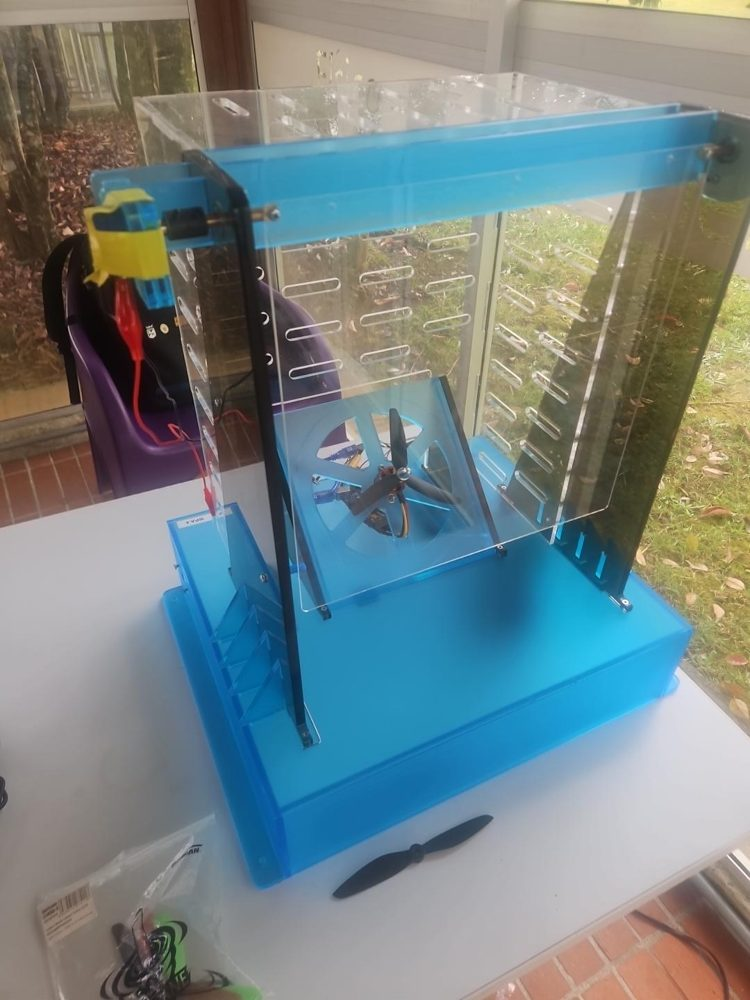
\includegraphics[width=\linewidth]{figs/mpa4_frente.jpg}\\[-1pt]{\scriptsize (a) vista frontal}
\end{minipage}\hfill
\begin{minipage}[t]{0.32\linewidth}\centering
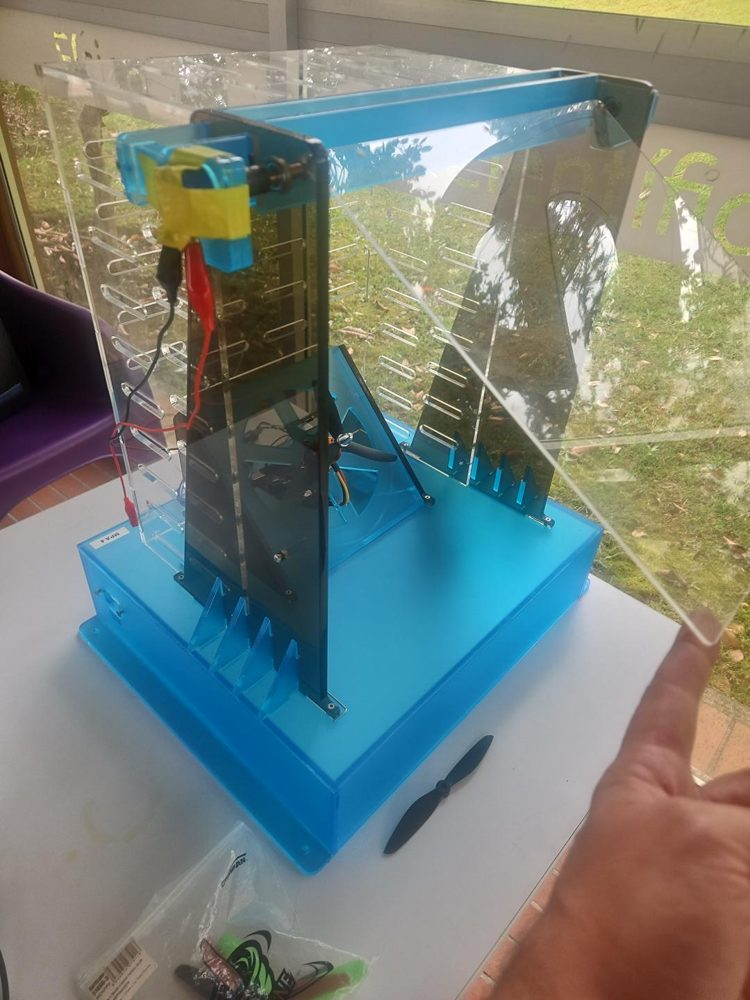
\includegraphics[width=\linewidth]{figs/mpa4_lamina.jpg}\\[-1pt]{\scriptsize (b) la lámina gira sobre el eje superior}
\end{minipage}\hfill
\begin{minipage}[t]{0.32\linewidth}\centering
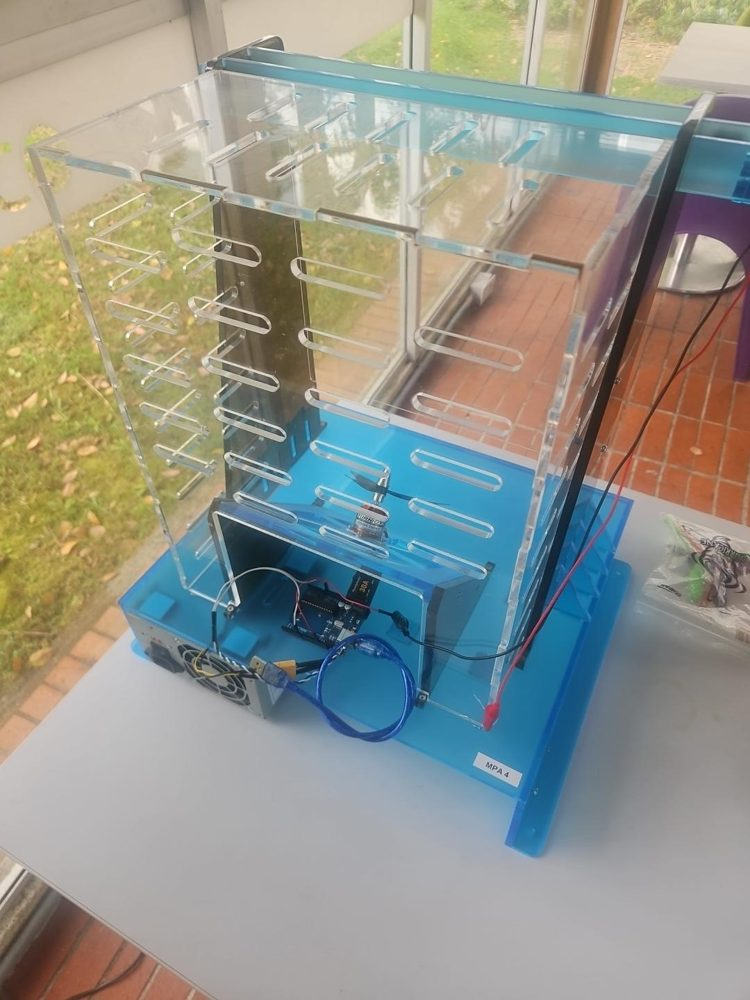
\includegraphics[width=\linewidth]{figs/mpa4_posterior.jpg}\\[-1pt]{\scriptsize (c) vista posterior}
\end{minipage}
\caption{La MPA 4. (a) La hélice, dentro de su protección inclinada, sopla hacia la lámina transparente; arriba a la izquierda, el potenciómetro (cinta amarilla) acoplado al eje. (b) La lámina cuelga del eje superior y el chorro la levanta. (c) Detrás: Arduino, ESC, motor y fuente ATX.}\label{fig:fotos}
\end{figure}

Una lámina de acrílico cuelga de un eje horizontal. Un motor \emph{brushless} mueve una hélice cuyo chorro empuja la lámina hacia arriba; la gravedad la devuelve y el aire y los rodamientos la frenan. Con el motor apagado, la lámina descansa en 0° contra su tope. Un potenciómetro acoplado al eje entrega una tensión que depende del ángulo.

\subsection{El modelo físico}

Visto desde el eje, es un péndulo con un empuje que depende de la velocidad de la hélice $\omega_h$ y del propio ángulo, porque al subir la lámina cambia cómo la golpea el chorro:
\begin{equation}
J\,\ddot\theta + b\,\dot\theta + \tau_g(\theta) = \tau_a(\theta,\omega_h),
\qquad
\tau_m\,\dot\omega_h = -\omega_h + g_m(u).
\label{eq:fisico}
\end{equation}
$J$ es la inercia de la lámina, $b$ el amortiguamiento (aire y rodamientos), $\tau_g$ el par de la gravedad, $\tau_a$ el par del chorro y $\tau_m$ la constante de tiempo del conjunto ESC--motor--hélice. Con el ángulo medido desde la vertical de reposo, $\tau_g = m g d\sin\theta$, y su pendiente $m g d\cos\theta$ se va a cero cerca de 90°: allá arriba la gravedad casi no devuelve la lámina.

\begin{figure}[H]\centering
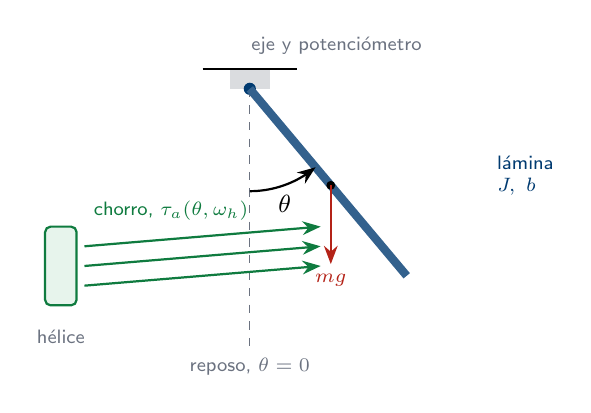
\begin{tikzpicture}[scale=1.0]
  \fill[gris!25] (-0.25,0) rectangle (0.25,0.25);
  \draw[thick] (-0.6,0.25) -- (0.6,0.25);
  \fill[azulEIA] (0,0) circle (2.2pt);
  \draw[dashed,gris] (0,0) -- (0,-3.3) node[below,lab]{reposo, $\theta=0$};
  \draw[line width=3pt,azulEIA!80] (0,0) -- ({3.1*sin(40)},{-3.1*cos(40)});
  \draw[->,thick] (0,-1.3) arc (-90:-50:1.3) node[midway,below,font=\small]{$\theta$};
  \coordinate (cg) at ({1.6*sin(40)},{-1.6*cos(40)});
  \fill (cg) circle (1.6pt);
  \draw[->,thick,rojoAviso] (cg) -- ++(0,-1.0) node[below,font=\scriptsize]{$mg$};
  \draw[blkv,minimum width=6mm] (-2.6,-2.75) rectangle (-2.2,-1.75);
  \node[lab,align=center] at (-2.4,-3.15) {hélice};
  \foreach \yy in {-2.0,-2.25,-2.5}{\draw[->,thick,verdeOK] (-2.1,\yy) -- (0.9,\yy+0.25);}
  \node[font=\scriptsize,verdeOK] at (-1.0,-1.55) {chorro, $\tau_a(\theta,\omega_h)$};
  \node[font=\scriptsize,azulEIA,align=left] at (3.5,-1.1) {lámina\\$J,\ b$};
  \node[lab] at (1.1,0.55) {eje y potenciómetro};
\end{tikzpicture}
\caption{Esquema (no a escala). El chorro levanta la lámina, la gravedad la devuelve. El equilibrio aparece donde los dos pares se igualan.}\label{fig:pendulo}
\end{figure}

\subsection{Por qué el modelo depende del punto de operación}

Alrededor de un equilibrio $(u_0,\theta_0)$, con desviaciones $\tilde\theta=\theta-\theta_0$ y $\tilde u=u-u_0$, la ecuación~\eqref{eq:fisico} se linealiza en
\begin{equation}
J\,\ddot{\tilde\theta} + b\,\dot{\tilde\theta} + k\,\tilde\theta = \kappa\,\tilde u,
\qquad
k = \left.\frac{\partial \tau_g}{\partial\theta}-\frac{\partial \tau_a}{\partial\theta}\right|_{0},
\label{eq:lineal}
\end{equation}
suponiendo que la hélice responde mucho más rápido que la lámina ($\tau_m$ pequeño). La rigidez $k$ y la ganancia $\kappa$ \textbf{cambian con $\theta_0$}: un modelo identificado cerca de 40° describe la planta cerca de 40°, no a 70°.

\begin{nota}[Dos no linealidades que no se deben confundir]
La curvatura del potenciómetro afecta la \emph{medición}; el cambio de $k$ y $\kappa$ con el ángulo afecta la \emph{planta}. La calibración corrige la primera. La segunda no desaparece: se maneja escogiendo un punto de operación y, si el reto lo pide, identificando más de uno.
\end{nota}

\subsection{Señales y magnitudes}

\begin{figure}[H]\centering
\resizebox{\linewidth}{!}{%
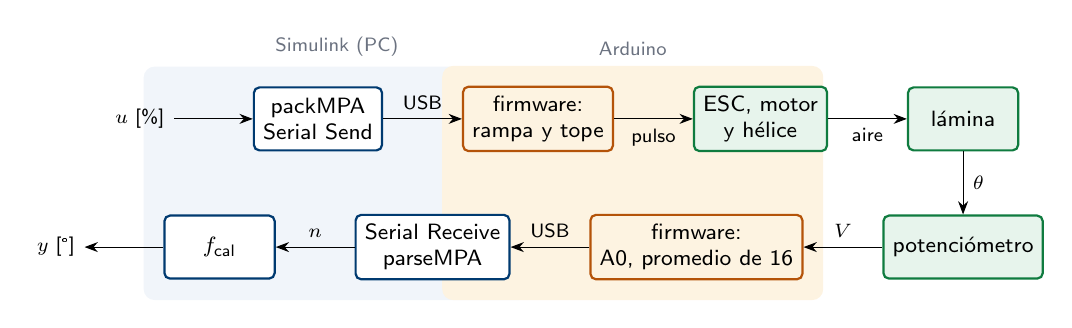
\begin{tikzpicture}[node distance=10mm]
  \node[sig] (u) {$u$ [\%]};
  \node[blkw,right=of u] (pk) {packMPA\\Serial Send};
  \node[blka,right=of pk] (fw) {firmware:\\rampa y tope};
  \node[blkv,right=of fw] (esc) {ESC, motor\\y hélice};
  \node[blkv,right=of esc] (lam) {lámina};
  \node[blkv,below=8mm of lam] (pot) {potenciómetro};
  \node[blka,left=of pot] (a0) {firmware:\\A0, promedio de 16};
  \node[blkw,left=of a0] (pr) {Serial Receive\\parseMPA};
  \node[blkw,left=of pr] (cal) {$f_\text{cal}$};
  \node[sig,left=of cal] (y) {$y$ [°]};
  \draw[->] (u) -- (pk); \draw[->] (pk) -- node[above,sig]{USB} (fw);
  \draw[->] (fw) -- node[below,sig]{pulso} (esc); \draw[->] (esc) -- node[below,sig]{aire} (lam);
  \draw[->] (lam) -- node[right,sig]{$\theta$} (pot); \draw[->] (pot) -- node[above,sig]{$V$} (a0);
  \draw[->] (a0) -- node[above,sig]{USB} (pr); \draw[->] (pr) -- node[above,sig]{$n$} (cal); \draw[->] (cal) -- (y);
  \begin{scope}[on background layer]
    \node[fill=azulClaro!60,rounded corners,fit=(pk)(pr)(cal),inner sep=2.5mm,label={[lab]above:Simulink (PC)}] {};
    \node[fill=ambarClaro,rounded corners,fit=(fw)(a0),inner sep=2.5mm,label={[lab]above:Arduino}] {};
  \end{scope}
\end{tikzpicture}}
\caption{Cadena completa de actuación y medida.}\label{fig:cadena}
\end{figure}

\begin{table}[H]\centering\small
\caption{Magnitudes que no deben confundirse.}\label{tab:magnitudes}
\rowcolors{2}{azulClaro}{white}
\begin{tabularx}{\linewidth}{@{}l l >{\raggedright\arraybackslash}X@{}}\toprule
\textbf{Símbolo} & \textbf{Unidad} & \textbf{Significado}\\\midrule
$u$ & \% & Mando que pide Simulink (0--100). Se convierte en un ancho de pulso para el ESC (sección~\ref{sec:escala}).\\
$u_\text{ap}$ & \% & Mando que el Arduino aplicó de verdad, después de la rampa y el tope. Lo reporta en cada paquete.\\
$p$ & \si{\micro s} & Ancho del pulso que recibe el ESC, cada \SI{20}{ms}.\\
$n$ & cuentas & Lectura del ADC en A0 (0--1023), promedio de 16 lecturas. Sale de \texttt{parseMPA} como \sen{adc}.\\
$\theta$, $y$ & ° & Ángulo físico de la lámina y su estimación a partir de $n$ con la calibración.\\
$u_0,\ \theta_0$ & \%, ° & Punto de operación: mando constante y ángulo de equilibrio que produce.\\
$\tilde u,\ \tilde\theta$ & \%, ° & Desviaciones respecto al punto de operación. El modelo lineal trabaja con ellas.\\\bottomrule
\end{tabularx}
\end{table}

% =====================================================================
\section{Conexiones y seguridad}\label{sec:conexiones}

\begin{figure}[H]\centering
\resizebox{\linewidth}{!}{%
\begin{circuitikz}[font=\normalsize, line width=0.7pt]
  \draw[thick,draw=azulEIA,fill=azulClaro,rounded corners=3pt] (0,0) rectangle (3,7);
  \node[azulEIA,font=\bfseries,align=center] at (1.5,6.5) {Arduino};
  \node[gris,font=\footnotesize,align=center] at (1.5,6.05) {UNO / Leonardo};
  \foreach \y/\n in {5.2/5V,4.0/A0,2.6/GND,1.2/D6}{
     \draw (2.75,\y) -- (3,\y); \node[anchor=east,font=\footnotesize\bfseries] at (2.7,\y) {\n};
     \fill (3,\y) circle (1.6pt);}
  \draw[thick] (0,3.6) -- (-1.4,3.6) node[left,align=right,font=\footnotesize]{USB\\al PC\\(Simulink)};
  \draw (3,5.2) -- (5.5,5.2) to[R, l_=\mbox{$R_s = 10\,\mathrm{k}\Omega$}, *-*] (5.5,4.0);
  \draw (3,4.0) -- (5.5,4.0);
  \draw (5.5,4.0) -- (6.6,4.0);
  \draw (7.4,4.9) to[pR, n=pot, mirror] (7.4,2.6);
  \draw (6.6,4.0) |- (pot.wiper);
  \draw (7.4,4.9) -- (7.4,5.15) node[ocirc]{} node[right,gris,font=\footnotesize]{sin conectar};
  \node[anchor=west,align=left,font=\footnotesize] at (7.75,3.8) {\textbf{potenciómetro}\\(gira con el eje)\\central $\to$ A0};
  \draw (3,2.6) -- (7.4,2.6); \node[font=\footnotesize,anchor=west] at (7.5,2.85) {extremo $\to$ GND};
  \node[azulEIA,font=\footnotesize\bfseries,anchor=south] at (6.2,5.45) {Sensor de posición};
  \draw[thick,draw=ambar,fill=ambar!8,rounded corners=3pt] (11.8,0.3) rectangle (14.2,2.3);
  \node[ambar,font=\bfseries,align=center] at (13,1.3) {ESC};
  \draw[thick,black!70] (3,1.2) -- (11.8,1.2) node[pos=0.55,above,black,font=\footnotesize]{señal del ESC (blanco o amarillo) $\to$ pin 6};
  \draw (11.8,0.65) -- (4.2,0.65) -- (4.2,2.6);  \fill (4.2,2.6) circle (1.6pt);
  \node[below,font=\footnotesize] at (6.8,0.65) {negro $\to$ GND del Arduino (tierra común)};
  \draw[rojoAviso] (11.8,1.85) -- (11,1.85) node[ocirc]{} node[left,font=\footnotesize,rojoAviso]{rojo: \textbf{NO} conectar};
  \draw[thick,draw=gris,fill=gris!10,rounded corners=3pt] (11.6,3.6) rectangle (14.4,5.0);
  \node[align=center,font=\footnotesize] at (13,4.3) {\textbf{Fuente ATX}\\12 V};
  \draw[very thick,ambar] (12.3,3.6) -- (12.3,2.3) node[pos=0.5,left,font=\footnotesize,black]{+12 V};
  \draw[very thick] (13.7,3.6) -- (13.7,2.3) node[pos=0.5,right,font=\footnotesize]{GND};
  \draw[thick,fill=white] (16.7,1.3) circle (0.55) node[font=\bfseries]{M};
  \foreach \y/\c in {1.85/A,1.3/B,0.75/C}{\draw (14.2,\y) -- (16.15,\y) node[pos=0.25,above,font=\scriptsize]{\c};}
  \node[align=center,font=\footnotesize,verdeOK] at (16.7,0.15) {intercambiar dos fases\\invierte el giro};
  \node[font=\footnotesize,anchor=south] at (16.7,1.9) {motor \emph{brushless}};
\end{circuitikz}}
\caption{Conexiones de la MPA.}\label{fig:conexiones}
\end{figure}

\begin{itemize}[leftmargin=12pt]
  \item \textbf{Sensor}: el terminal central del potenciómetro va a \textbf{A0}; de A0 sale una resistencia de 10~k$\Omega$ hacia \textbf{5~V}; un extremo del potenciómetro va a \textbf{GND} y el otro queda libre. A0 ve el divisor $V_{A0}=5\,\text{V}\cdot R_\text{pot}(\theta)/(R_\text{pot}(\theta)+R_s)$, que \textbf{no es lineal} en $\theta$: por eso se calibra (sección~\ref{sec:sensor}).
  \item \textbf{Señal del ESC}: del cable de tres hilos del ESC, el de \textbf{señal} (blanco o amarillo) va al \textbf{pin 6} y el \textbf{negro} a GND del Arduino. Sin esa tierra común el ESC no entiende la señal. El \textbf{rojo no se conecta}. \ficha
  \item \textbf{Potencia}: el ESC se alimenta de los 12~V de la fuente ATX (amarillo) y su GND (negro). El Arduino se alimenta y se comunica por USB.
  \item \textbf{Motor}: el ESC sale al motor por tres cables. Su orden solo decide el sentido de giro; \textbf{intercambiar dos cualesquiera lo invierte} (sección~\ref{sec:helice}).
\end{itemize}

\begin{peligro}[Seguridad: antes de cada ensayo]
\begin{itemize}[leftmargin=12pt]
  \item Manos, cabello, cables y objetos lejos de la hélice y del recorrido de la lámina. \textbf{Nunca} se toca la lámina ni la hélice con la fuente encendida.
  \item La fuente se enciende con el modelo de Simulink ya corriendo y $u=0$; se apaga antes de detenerlo.
  \item Si el motor se calienta, vibra de forma anormal o la fuente se protege, paren el ensayo. Una fuente ATX protegida no vuelve sola: hay que desconectarla de la red unos segundos y volver a conectarla.
  \item Revisen que la lámina no esté doblada y que los tornillos estén firmes. Una lámina doblada cambia el modelo.
\end{itemize}
\end{peligro}

% =====================================================================
\section{La hélice: montaje y sentido de giro}\label{sec:helice}

\begin{figure}[H]\centering
\begin{minipage}[t]{0.23\linewidth}\centering
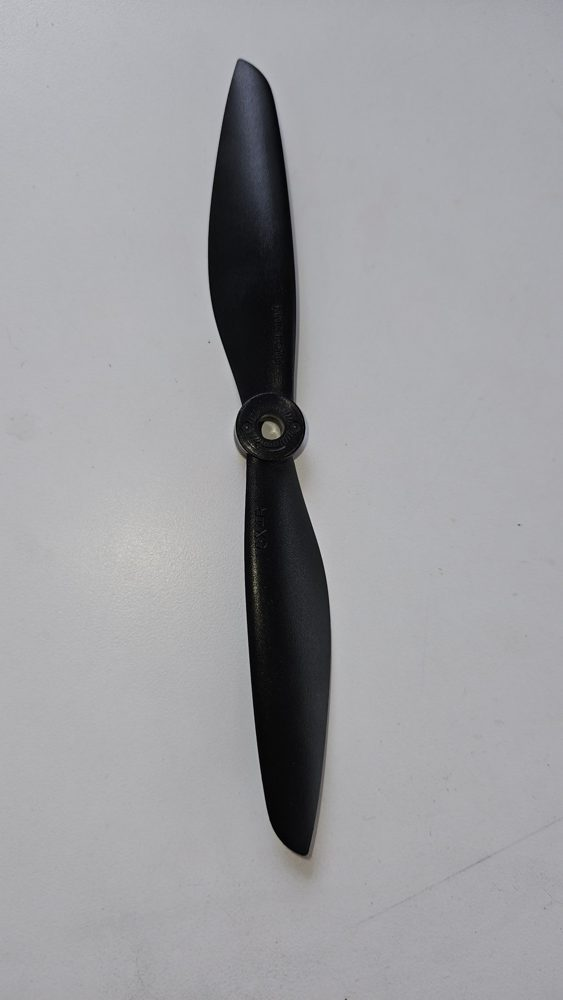
\includegraphics[width=\linewidth]{figs/helice_cara_6x45.jpg}\\[-1pt]{\scriptsize (a) cara con el tamaño (6×4.5)}
\end{minipage}\hfill
\begin{minipage}[t]{0.23\linewidth}\centering
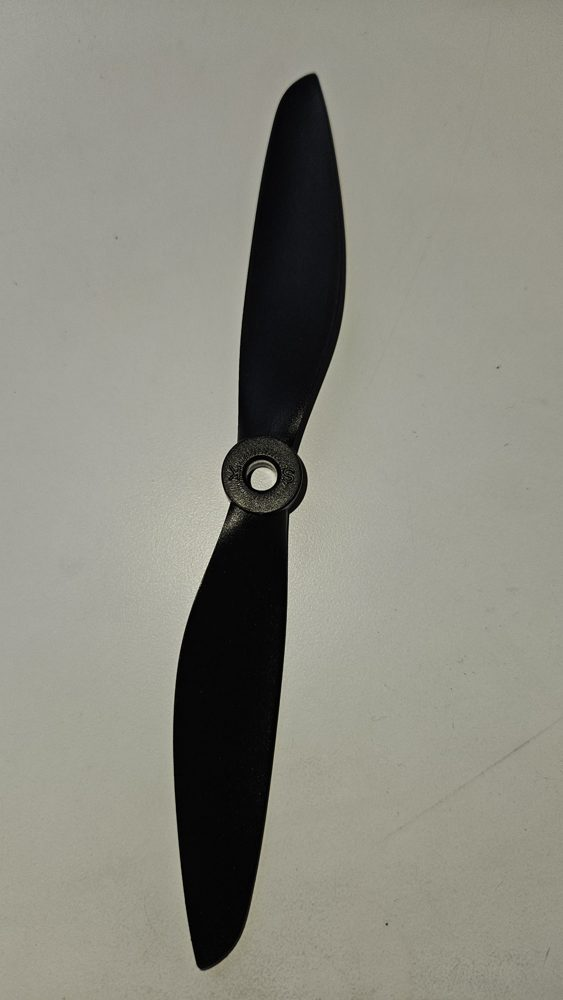
\includegraphics[width=\linewidth]{figs/helice_cara_SK.jpg}\\[-1pt]{\scriptsize (b) cara opuesta (marca)}
\end{minipage}\hfill
\begin{minipage}[t]{0.23\linewidth}\centering
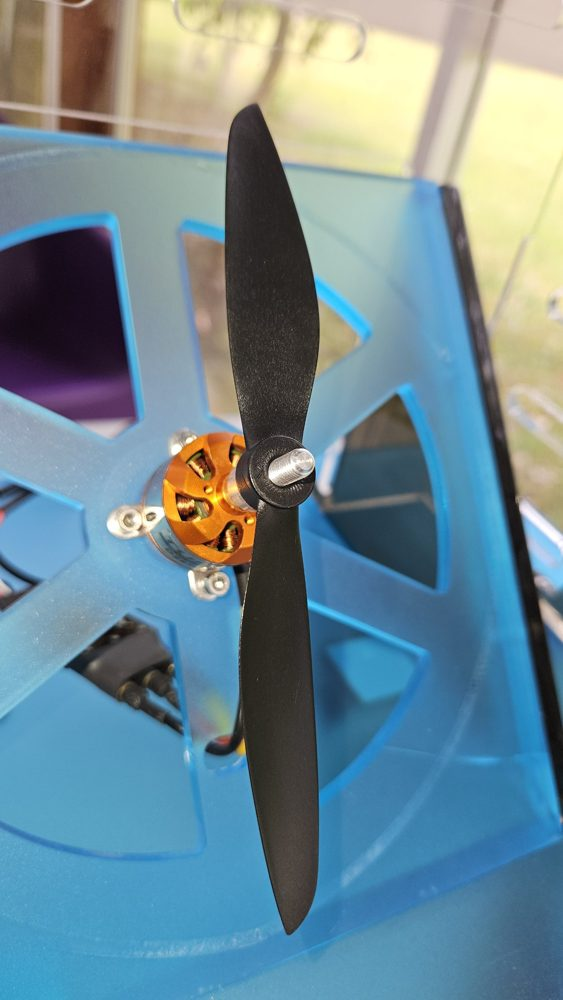
\includegraphics[width=\linewidth]{figs/helice_montada_lado.jpg}\\[-1pt]{\scriptsize (c) montada en la MPA 4}
\end{minipage}\hfill
\begin{minipage}[t]{0.23\linewidth}\centering
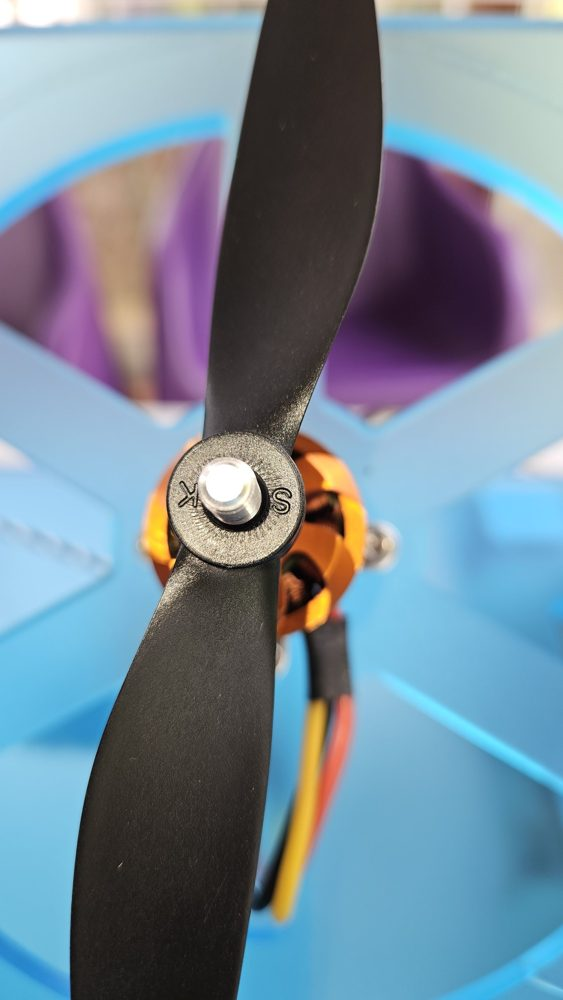
\includegraphics[width=\linewidth]{figs/helice_montada_frente.jpg}\\[-1pt]{\scriptsize (d) detalle del montaje}
\end{minipage}
\caption{Hélice 6×4.5 y su montaje en la MPA 4, que funcionó después de corregir la orientación y el sentido de giro.}\label{fig:helice}
\end{figure}

Una hélice no es simétrica: tiene una cara que empuja el aire y un sentido de giro para el que está diseñada (algunas lo indican con una flecha o marcas en el cubo). Con la hélice al revés o girando al revés, el motor gira, hace ruido y la lámina apenas se mueve. Es el error más difícil de ver y el que más tiempo hace perder.

\begin{cuidado}[La regla: el aire tiene que ir hacia la lámina]
Piensen en un dron: para despegar, sus hélices empujan el aire hacia el \textbf{piso}. En la MPA el «piso» es la \textbf{lámina}: la hélice se monta de manera que la cara que en un dron miraría al piso mire hacia la lámina. Si una hélice venía montada al contrario, la planta no levanta la lámina aunque todo lo demás esté bien.
\end{cuidado}

\begin{pasos}[Verificación del sentido del aire (cada vez que se cambie o se desmonte la hélice)]
\begin{enumerate}[leftmargin=14pt]
  \item Monten la hélice con la orientación de la regla anterior y aprieten la tuerca.
  \item Con el modelo corriendo y el motor armado (sección~\ref{sec:enlace}), lleven $u$ a un valor bajo, \textbf{alrededor de 20\,\%}.
  \item Comprueben hacia dónde va el aire con una tira de papel sostenida \textbf{lejos} de la hélice, entre la protección y la lámina. Nunca con la mano.
  \item Si el aire \textbf{no} va hacia la lámina: $u=0$, apaguen la fuente, \textbf{intercambien dos de los tres cables} entre el ESC y el motor y repitan.
  \item Con el aire hacia la lámina, la lámina debe empezar a despegarse con un mando bajo (en la MPA 4, cerca de $u=10\,\%$). \ficha
\end{enumerate}
\end{pasos}

\begin{nota}[Por qué funciona este orden]
Con la hélice bien orientada, de los dos sentidos de giro solo uno manda el aire hacia la lámina, y es justamente el sentido para el que la hélice está diseñada. Si la hélice estuviera volteada, el giro que manda aire hacia la lámina sería el «equivocado» y el empuje sería pobre. Por eso primero se fija la orientación y después se corrige el giro con los cables.
\end{nota}

% =====================================================================
\section{El enlace con Simulink}\label{sec:enlace}

Simulink no maneja la MPA directamente. Un \textbf{firmware propio} en el Arduino hace el trabajo de tiempo real (medir, aplicar el pulso al ESC, proteger) y conversa con Simulink por el USB con paquetes binarios. Simulink calcula el controlador y envía el mando. No hace falta entender cada línea del código; sí hace falta saber qué hace, porque dos de sus funciones (la rampa y el tope) son parte del actuador que se va a modelar.

\subsection{Qué hace el firmware}

\begin{figure}[H]\centering
\resizebox{0.96\linewidth}{!}{%
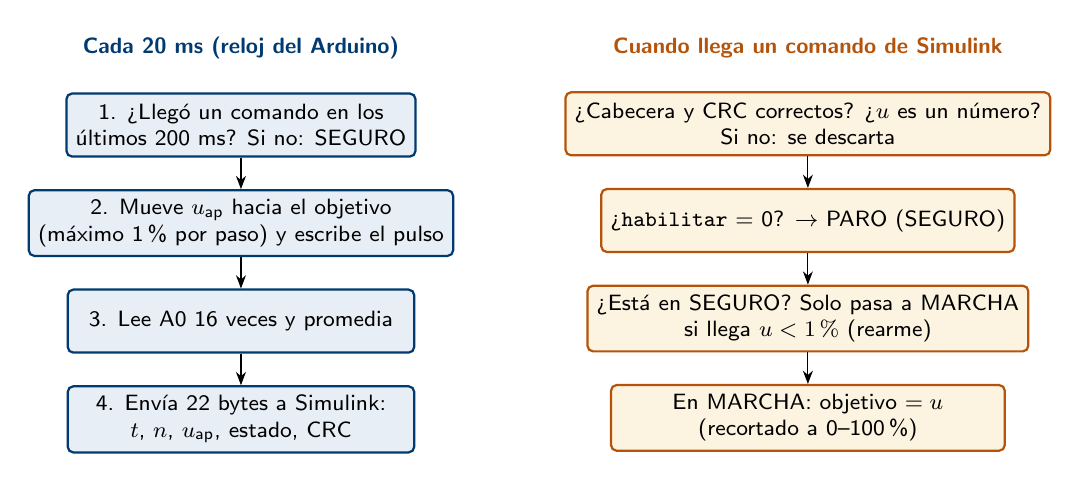
\begin{tikzpicture}[node distance=4mm]
  \node[font=\footnotesize\bfseries,color=azulEIA] (t1) at (0,0) {Cada 20 ms (reloj del Arduino)};
  \node[blk,below=3mm of t1,minimum width=44mm] (w) {1. ¿Llegó un comando en los\\últimos 200 ms? Si no: SEGURO};
  \node[blk,below=of w,minimum width=44mm] (r) {2. Mueve $u_\text{ap}$ hacia el objetivo\\(máximo 1\,\% por paso) y escribe el pulso};
  \node[blk,below=of r,minimum width=44mm] (a) {3. Lee A0 16 veces y promedia};
  \node[blk,below=of a,minimum width=44mm] (s) {4. Envía 22 bytes a Simulink:\\$t$, $n$, $u_\text{ap}$, estado, CRC};
  \draw[->] (w)--(r); \draw[->] (r)--(a); \draw[->] (a)--(s);
  \node[font=\footnotesize\bfseries,color=ambar] (t2) at (7.2,0) {Cuando llega un comando de Simulink};
  \node[blka,below=3mm of t2,minimum width=50mm] (c) {¿Cabecera y CRC correctos? ¿$u$ es un número?\\Si no: se descarta};
  \node[blka,below=of c,minimum width=50mm] (p) {¿\texttt{habilitar} = 0? $\to$ PARO (SEGURO)};
  \node[blka,below=of p,minimum width=50mm] (q) {¿Está en SEGURO? Solo pasa a MARCHA\\si llega $u<1\,\%$ (rearme)};
  \node[blka,below=of q,minimum width=50mm] (o) {En MARCHA: objetivo $=u$\\(recortado a 0--100\,\%)};
  \draw[->] (c)--(p); \draw[->] (p)--(q); \draw[->] (q)--(o);
\end{tikzpicture}}
\caption{Las dos tareas del firmware. El estado SEGURO lleva el mando a 0 (en rampa) y espera un rearme.}\label{fig:firmware}
\end{figure}

\begin{table}[H]\centering\small
\caption{Parámetros del firmware (al inicio de \texttt{MPA\_Firmware.ino}). Los que cambian por unidad van a la ficha.}\label{tab:parametros}
\rowcolors{2}{azulClaro}{white}
\begin{tabularx}{\linewidth}{@{}>{\ttfamily}l l >{\raggedright\arraybackslash}X@{}}\toprule
\normalfont\textbf{Parámetro} & \textbf{Valor} & \textbf{Qué hace}\\\midrule
PIN\_ESC & 6 & Pin de la señal del ESC. \ficha\\
PERIODO\_US & 20000 & Periodo del lazo: \SI{20}{ms} = 50~Hz. Es el $T_s$ de Simulink.\\
PULSO\_0 & 1000 \si{\micro s} & Pulso con $u=0$: motor detenido y pulso de armado del ESC.\\
PULSO\_100 & 1450 \si{\micro s} & Pulso con $u=100\,\%$: máxima velocidad útil. \ficha\\
PULSO\_TOPE & 1450 \si{\micro s} & Ningún pulso lo supera, aunque Simulink pida más. \ficha\\
RAMPA\_PCT\_S & 50 \%/s & Rapidez máxima de cambio del mando aplicado (1\,\% por paso).\\
TIMEOUT\_MS & 200 & Sin comandos válidos por ese tiempo, el mando baja a 0.\\
U\_REARME & 1 \% & Después de SEGURO, el motor solo arranca si llega $u$ menor que esto.\\
N\_ADC & 16 & Lecturas de A0 promediadas por muestra.\\\bottomrule
\end{tabularx}
\end{table}

\subsection{Cargar el firmware}\label{sec:firmware}

El archivo está en el repositorio del curso, carpeta \texttt{firmware/MPA\_Firmware/}. La carpeta y el archivo \texttt{.ino} deben llamarse igual, como exige el Arduino IDE.

\begin{pasos}[Grabar el firmware (una vez por unidad, o cuando alguien lo haya borrado)]
\begin{enumerate}[leftmargin=14pt]
  \item Fuente del ESC \textbf{apagada}. Conecten el Arduino por USB.
  \item Abran \texttt{MPA\_Firmware.ino} con el Arduino IDE (2.x o 1.8.x). No hace falta instalar librerías: \texttt{Servo} viene con el IDE.
  \item \emph{Tools $\to$ Board}: \textbf{Arduino Uno} o \textbf{Arduino Leonardo}, según su unidad. \emph{Tools $\to$ Port}: el COM del Arduino. \ficha
  \item Revisen al inicio del archivo \texttt{PIN\_ESC} (6) y, si la ficha lo indica, \texttt{PULSO\_100} y \texttt{PULSO\_TOPE}.
  \item \emph{Upload} (flecha $\to$). Debe terminar con «Done uploading». Si el puerto está ocupado, cierren MATLAB y el monitor serie.
  \item \textbf{Cierren el monitor serie del IDE} antes de abrir Simulink: si queda abierto, ocupa el puerto. (Si lo abren, verán símbolos raros: los paquetes son binarios, no texto.)
  \item Peguen en la unidad el rótulo «Firmware MPA v2: no usar Connected IO».
\end{enumerate}
\end{pasos}

\begin{nota}[¿Cómo sé que el firmware está bien?]
Con el modelo de Simulink corriendo y la fuente apagada: \sen{valido} $=1$, \sen{estado} pasa a 1 con $u=0$, \sen{diff(t_ard)} $=0.02$ y \sen{adc} cambia al mover la lámina con la mano. Si Simulink se queda esperando y da \emph{timeout}, el Arduino no tiene este firmware o el puerto es otro.
\end{nota}

\subsection{El subsistema MPA en Simulink}

Todo el enlace se encapsula en un subsistema \blq{MPA}: entra el mando, salen las medidas. Es el mismo esquema que se usó con la bomba de infusión de Biomecatrónica.

\begin{figure}[H]\centering
\resizebox{\linewidth}{!}{%
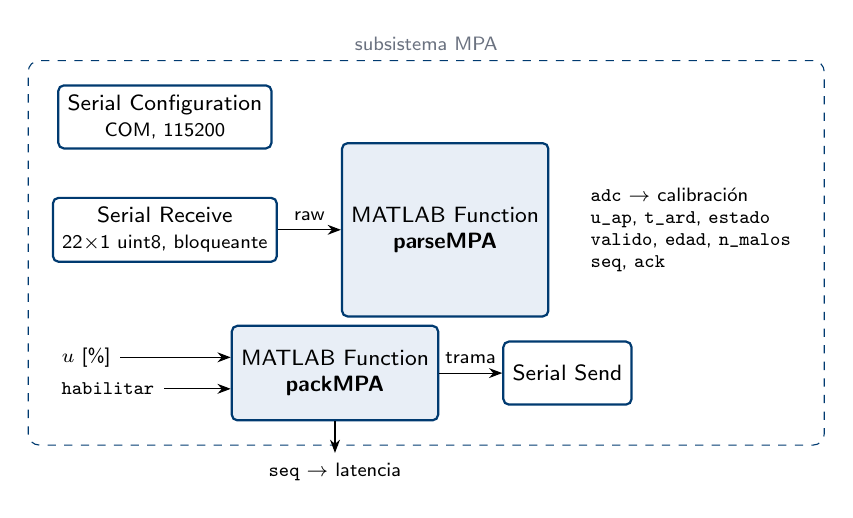
\begin{tikzpicture}[node distance=6mm]
  \node[blkw] (cfg) {Serial Configuration\\\scriptsize COM, 115200};
  \node[blkw,below=6mm of cfg] (rx) {Serial Receive\\\scriptsize 22$\times$1 uint8, bloqueante};
  \node[blk,right=8mm of rx,minimum height=22mm,minimum width=26mm] (pa) {MATLAB Function\\\textbf{parseMPA}};
  \node[sig,anchor=west,align=left] at ($(pa.east)+(4mm,0)$) (outs) {\sen{adc} $\to$ calibración\\\sen{u_ap}, \sen{t_ard}, \sen{estado}\\\sen{valido}, \sen{edad}, \sen{n_malos}\\\sen{seq}, \sen{ack}};
  \node[sig,below=12mm of rx.south west,anchor=west] (u) {$u$ [\%]};
  \node[sig,below=4mm of u.west,anchor=west] (h) {\texttt{habilitar}};
  \node[blk,right=14mm of u,yshift=-2mm,minimum height=12mm,minimum width=26mm] (pk) {MATLAB Function\\\textbf{packMPA}};
  \node[blkw,right=8mm of pk] (tx) {Serial Send};
  \draw[->] (rx) -- node[above,sig]{raw} (pa);
  \draw[->] (u) -- ($(pk.west)+(0,2mm)$); \draw[->] (h) -| ($(pk.west)+(-3mm,-2mm)$) -- ($(pk.west)+(0,-2mm)$);
  \draw[->] (pk) -- node[above,sig]{trama} (tx);
  \draw[->] (pk.south) -- ++(0,-4mm) node[below,sig]{\sen{seq} $\to$ latencia};
  \begin{scope}[on background layer]
    \node[draw=azulEIA,dashed,rounded corners,fit=(cfg)(rx)(pa)(pk)(tx)(outs),inner sep=3mm,label={[lab]above:subsistema MPA}] {};
  \end{scope}
\end{tikzpicture}}
\caption{Subsistema \blq{MPA}. Los bloques seriales son del \emph{Instrument Control Toolbox}; el código de las dos MATLAB Function está en los archivos \texttt{parseMPA.m} y \texttt{packMPA.m}.}\label{fig:subsistema}
\end{figure}

\begin{table}[H]\centering\small
\caption{Configuración de los bloques y del modelo.}\label{tab:config}
\rowcolors{2}{azulClaro}{white}
\begin{tabularx}{\linewidth}{@{}l >{\raggedright\arraybackslash}X@{}}\toprule
\textbf{Dónde} & \textbf{Valor}\\\midrule
Serial Configuration & Puerto COM de la unidad, 115200, 8 bits, sin paridad, 1 de parada, sin control de flujo, \emph{Timeout} 5~s. \ficha\\
Serial Receive & \emph{Header} vacío, \emph{Terminator} \texttt{<none>}, \emph{Data size} \texttt{[22 1]}, \emph{Data type} \texttt{uint8}, \textbf{\emph{Enable blocking mode} activado}, \emph{Block sample time} 0.02.\\
Serial Send & \emph{Header} vacío, \emph{Terminator} \texttt{<none>}.\\
MATLAB Function & Pegar el contenido \emph{completo} de cada \texttt{.m}, con sus funciones auxiliares del final. En \emph{Edit Data}, las salidas de \texttt{parseMPA} con tipo \emph{Inherit} o \texttt{double}: si \sen{u_ap} queda en \texttt{uint8}, pierde los decimales y el lazo del Reto~3 no puede restarla de un \texttt{double}.\\
Solver & Paso fijo, \texttt{ode4} (o \texttt{ode1}), $T_s=0.02$~s. No \texttt{discrete}: el controlador y el observador del Reto 3 son bloques continuos. Stop time según el ensayo.\\
Simulation Pacing & \textbf{Apagado}: el Arduino marca el paso (ver abajo).\\
Hardware board & \texttt{None}.\\
Data Import/Export & \emph{Single simulation output} \textbf{desmarcado} y \emph{Time} (\sen{tout}) marcado: cada \blq{To Workspace} deja su variable suelta en el workspace, sin \sen{out}.\\\bottomrule
\end{tabularx}
\end{table}

\begin{nota}[Por qué el tiempo de Simulink es tiempo real]
El \blq{Serial Receive} bloqueante espera a que llegue cada paquete, y el Arduino envía uno cada \SI{20}{ms} con su propio reloj. Simulink avanza entonces exactamente un paso de \SI{0.02}{s} por paquete: el tiempo de simulación \emph{es} el tiempo del Arduino. Si el PC se retrasa, los paquetes esperan en el puerto y Simulink los consume más rápido hasta ponerse al día. Con \emph{Simulation Pacing} activado ese atraso no se recuperaría nunca.
\end{nota}

\subsection{La escala del mando}\label{sec:escala}

El ESC recibe la señal estándar de servo: un pulso cada \SI{20}{ms}, de \SI{1}{ms} (5\,\% del periodo) a \SI{2}{ms} (10\,\%). En la MPA el motor llega a su máxima velocidad útil mucho antes de \SI{2}{ms}, así que el firmware reparte el 0--100\,\% solo en la franja útil:
\begin{equation}
p = 1000 + \frac{u}{100}\,(1450-1000)\ \si{\micro s} = 1000 + 4.5\,u\ \si{\micro s}.
\label{eq:escala}
\end{equation}

\begin{table}[H]\centering\small
\caption{Escala del mando en la MPA 4 (comprueben la suya).}\label{tab:escala}
\rowcolors{2}{azulClaro}{white}
\begin{tabular}{@{}r r r >{\raggedright\arraybackslash}p{7cm}@{}}\toprule
$u$ [\%] & $p$ [\si{\micro s}] & duty [\%] & Qué pasa\\\midrule
0 & 1000 & 5.0 & Motor detenido; pulso de armado.\\
$\approx$7 & $\approx$1030 & 5.2 & Empieza a girar la hélice ($u_\text{arr}$).\\
$\approx$10 & $\approx$1045 & 5.2 & La lámina se despega del tope ($u_\text{mov}$).\\
100 & 1450 & 7.3 & Máxima velocidad útil; la lámina pasa de 90°.\\\bottomrule
\end{tabular}
\end{table}

\subsection{Rampa y tope: dos no linealidades del actuador}\label{sec:rampa}

\begin{itemize}[leftmargin=12pt]
  \item \textbf{Rampa}. El mando aplicado cambia como máximo 50\,\%/s (1\,\% por paso). Sin ella, un cambio brusco del mando hacía que el motor pidiera un pico de corriente al acelerar o devolviera energía a los 12~V al frenar, y la fuente ATX se protegía. La rampa es un \textbf{limitador de rapidez} ($|\dot u_\text{ap}|\le 50\,\%/\text{s}$): una no linealidad que solo actúa cuando se pide un cambio grande y rápido. Para cambios pequeños alrededor del punto de operación no se activa, y el modelo lineal sigue valiendo.
  \item \textbf{Tope}. Ningún pulso supera \texttt{PULSO\_TOPE}; junto con el recorte de $u$ a 0--100\,\% es una \textbf{saturación}.
\end{itemize}

\begin{cuidado}[Qué consecuencias tiene para el control]
\begin{itemize}[leftmargin=12pt]
  \item El lazo simulado lleva un \blq{Rate Limiter} de $\pm50$\,\%/s y una \blq{Saturation} antes del modelo de la planta; si no, lo simulado y lo real se separan en los cambios grandes.
  \item El Arduino reporta $u_\text{ap}$, el mando que de verdad recibió el ESC después de la rampa y del tope. Esa es la señal que un controlador con estados internos debe seguir (sección~\ref{sec:lazo}).
  \item En la identificación, el pulso de mando sale «redondeado» por la rampa. Por eso el análisis empieza cuando la rampa terminó de bajar (sección~\ref{sec:pulsos}).
\end{itemize}
\end{cuidado}

\subsection{Armado, rearme y PARO}

\begin{pasos}[Secuencia de arranque (siempre la misma)]
\begin{enumerate}[leftmargin=14pt]
  \item Fuente \textbf{apagada}. Modelo con $u=0$ y \texttt{habilitar} $=1$. \emph{Run}.
  \item Comprueben en Simulink: \sen{estado} $=1$, \sen{valido} $=1$, latencia 0 o 1.
  \item \textbf{Ahora} enciendan la fuente: suena la secuencia corta de armado y el ESC queda en silencio. Desde que el Arduino arranca envía el pulso de \SI{1000}{\micro s}, así que el ESC arma siempre que la fuente se encienda con el Arduino ya funcionando.
  \item Para terminar: $u=0$, esperen a que la hélice pare, apaguen la fuente y detengan Simulink.
\end{enumerate}
\end{pasos}

\begin{itemize}[leftmargin=12pt]
  \item \textbf{PARO}: \texttt{habilitar} $=0$ (un \blq{Manual Switch} entre dos constantes) lleva el mando a 0 en rampa.
  \item \textbf{Rearme}: después de un PARO, de un corte de comunicación o del arranque, el motor solo vuelve a moverse cuando llega un $u<1\,\%$. Si el modelo arranca con $u\ne0$, el motor no se mueve y \sen{estado} se queda en 0: no es una falla.
  \item \textbf{Corte de comunicación}: si Simulink se detiene o el cable se suelta, a los \SI{200}{ms} el mando baja solo a 0.
\end{itemize}

\subsection{Diagnóstico del enlace}

\begin{itemize}[leftmargin=12pt]
  \item \textbf{Latencia} $=\operatorname{mod}(\text{seq}_{k-1}-\text{ack}_k,\,65536)$: el número del comando anterior (salida \sen{seq} de \texttt{packMPA} por un \blq{Unit Delay}) menos el último que el Arduino aceptó (\sen{ack}). Debe ser 0 o 1. Si crece, el PC no alcanza los 50~Hz: cierren Scopes y quiten Displays.
  \item \sen{diff(t_ard)} debe valer 0.02 en todos los pasos; \sen{valido} en 1; \sen{n_malos} en 0 o casi.
\end{itemize}

% =====================================================================
\section{El sensor: de cuentas a grados}\label{sec:sensor}

\begin{figure}[H]\centering
\begin{minipage}[c]{0.26\linewidth}\centering
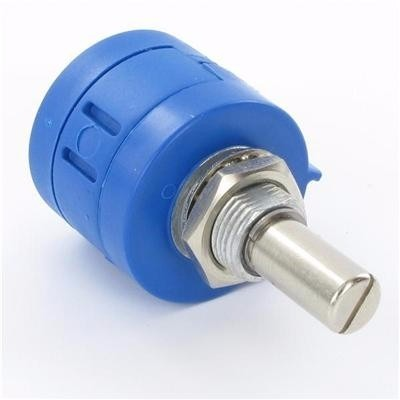
\includegraphics[width=0.85\linewidth]{figs/potenciometro.jpg}
\end{minipage}\hfill
\begin{minipage}[c]{0.70\linewidth}
La salida \sen{adc} de \texttt{parseMPA} ya está en cuentas (promedio de 16 lecturas, tipo \emph{double}), así que se calibra \textbf{directamente de cuentas a grados}, $\theta=f_\text{cal}(n)$: no hace falta la ganancia de voltios ni un \blq{Data Type Conversion}. La relación no es lineal (sección~\ref{sec:conexiones}) y puede subir o bajar al levantar la lámina según cómo esté montado el potenciómetro. Varias unidades tienen potenciómetros de reemplazo: miren la referencia impresa en el suyo. \ficha
\end{minipage}
\caption{Potenciómetro multivuelta típico (ilustración).}\label{fig:pot}
\end{figure}

\subsection{Calibración con el motor apagado}

\begin{pasos}[Procedimiento]
\begin{enumerate}[leftmargin=14pt]
  \item Fuente del ESC \textbf{apagada}. Modelo con el subsistema \blq{MPA}, \sen{adc} a un \blq{Display} y a un \blq{To Workspace}. \emph{Run}.
  \item Muevan la lámina con la mano despacio: la lectura debe cambiar en forma suave y repetible.
  \item Lleven la lámina a 0, 10, \dots, 90° según el indicador, \textbf{subiendo}. Esperen unos segundos en cada marca y anoten \sen{adc}. Repitan \textbf{bajando} (hoja de campo, anexo~\ref{sec:hojas}).
  \item Anoten además tres marcas \textbf{que no van a usar para ajustar} (15, 45 y 75°): son para validar.
\end{enumerate}
\end{pasos}

\begin{nota}[Medir el ángulo con el celular]
Si el indicador de su módulo está borroso, flojo o no tiene todas las marcas, usen una app de \textbf{nivel o inclinómetro} en el celular. En iPhone, la app \emph{Medidas} trae un nivel; en Android sirve cualquier app de nivel de burbuja o clinómetro.
\begin{enumerate}[leftmargin=14pt]
  \item Calibren la app sobre una mesa horizontal, si la app lo permite.
  \item Con la lámina \textbf{colgando en reposo}, apoyen el celular de canto contra su cara plana y anoten la lectura: ese es el 0° de su lámina. Lo que importa es el cambio desde ahí, no el número absoluto.
  \item Para cada marca, sostengan la lámina con una mano y el celular contra ella con la otra, sin empujar el eje. Lean el ángulo cuando la lectura esté quieta y anoten \sen{adc} al mismo tiempo.
  \item Usen siempre la misma cara de la lámina y la misma orientación del celular.
\end{enumerate}
Con esto la incertidumbre es de 1° aproximadamente, del orden del error de ajuste que se acepta. Si el indicador y la app no coinciden en más de 2°, confíen en la app y avisen al laboratorio.
\end{nota}

\subsection{El ajuste en MATLAB}

El guion \texttt{calibracion\_sensor.m} (carpeta \texttt{scripts/} del repositorio) hace todo el ajuste: solo hay que copiar las lecturas de la hoja de campo en su sección \texttt{DATOS} y ejecutarlo (F5).

\needspace{10\baselineskip}
\begin{lstlisting}[caption={La única parte que se edita en \texttt{calibracion\_sensor.m}.}]
%% DATOS (llenar con SU modulo)
modulo  = 4;                    % numero de la MPA
theta   = 0:10:90;              % marcas del indicador [grados]
n_sub   = [ ];                  % adc subiendo  (10 valores, uno por marca)
n_baj   = [ ];                  % adc bajando   (10 valores, uno por marca)
theta_v = [15 45 75];           % marcas de validacion (NO se usan en el ajuste)
n_v     = [ ];                  % adc en esas marcas (3 valores; puede quedar vacio)
\end{lstlisting}

El guion:
\begin{enumerate}[leftmargin=14pt]
  \item revisa que la lectura sea monótona y que la histéresis no pase de 5 cuentas;
  \item ajusta una recta y una cuadrática, y \textbf{escoge la recta si su error máximo es menor a 1°}; si no, la cuadrática;
  \item calcula el error en las marcas de validación, grafica los ajustes y el error en cada marca;
  \item escribe los coeficientes como $y = a_2\,n^2 + a_1\,n + a_0$ (con $a_2=0$ si es lineal) y los guarda, con el error, la histéresis, la resolución y la fecha, en \texttt{cal\_MPAxx.mat}. \ficha
\end{enumerate}

\begin{figure}[H]\centering
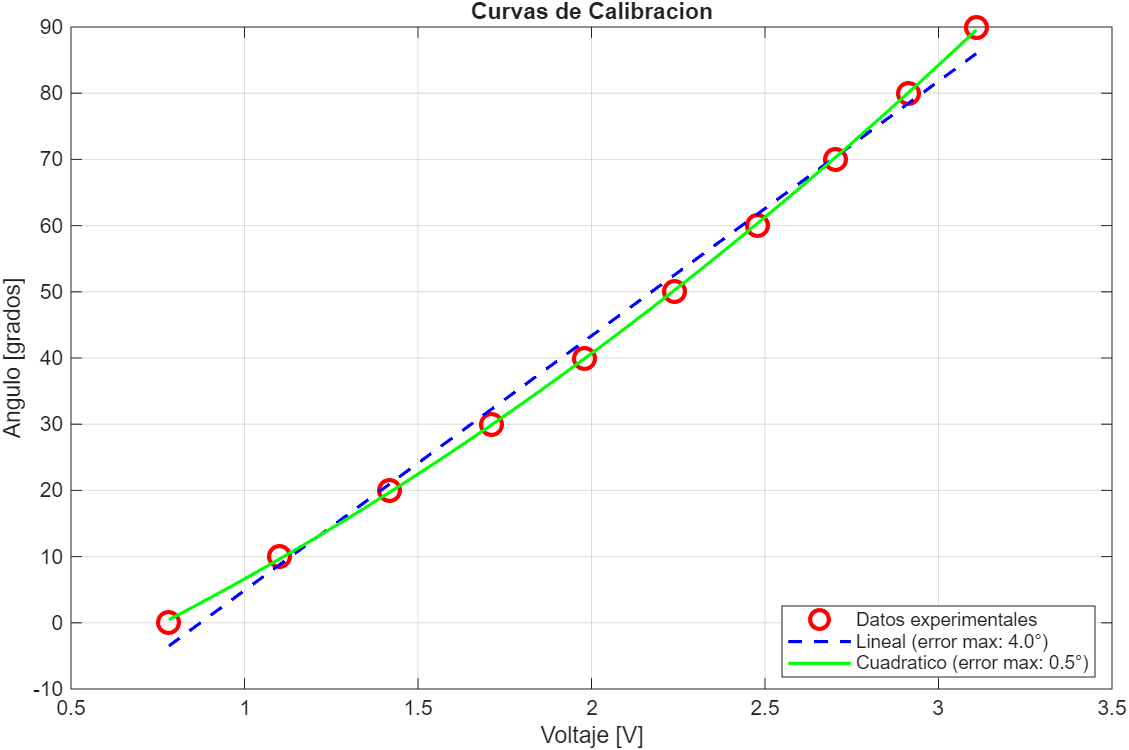
\includegraphics[width=0.52\linewidth]{figs/curvas_calibracion.png}
\caption{Ejemplo de la guía de 2026-1 (en voltios, una unidad): la recta deja errores de 4° y la cuadrática de 0.5°. En cuentas la forma es la misma; los coeficientes son los de su módulo.}\label{fig:curvas}
\end{figure}

\subsection{Llevar la calibración a Simulink}\label{sec:calsimulink}

Los coeficientes no se copian a mano en los bloques: los bloques usan los \emph{nombres} \texttt{a2}, \texttt{a1} y \texttt{a0}, y el modelo carga el archivo \texttt{cal\_MPAxx.mat} cada vez que arranca.

\begin{figure}[H]\centering
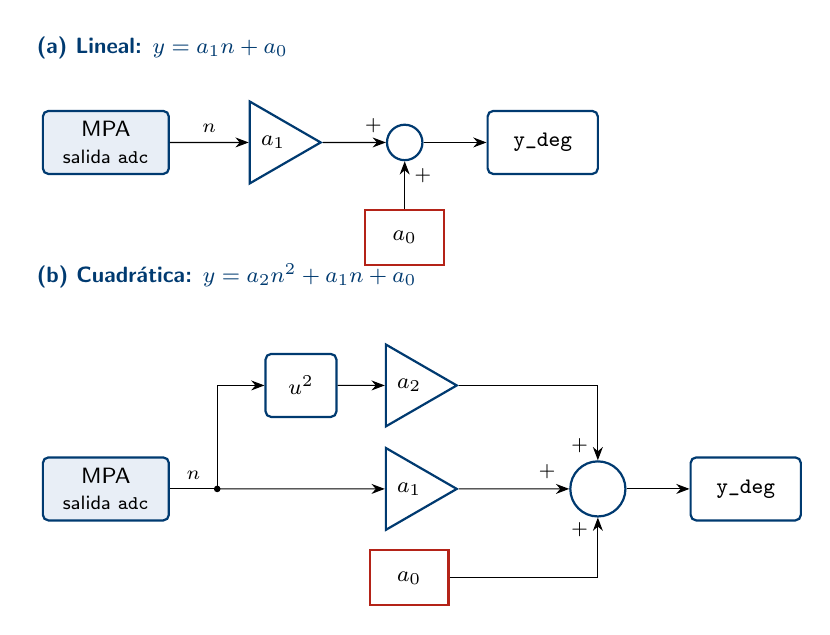
\begin{tikzpicture}[node distance=7mm,
   gain/.style={draw=azulEIA,thick,fill=white,isosceles triangle,isosceles triangle apex angle=60,minimum size=9mm,inner sep=1pt,font=\footnotesize},
   cte/.style={draw=rojoAviso,thick,fill=white,minimum width=10mm,minimum height=7mm,font=\footnotesize}]
  % --- lineal
  \node[font=\footnotesize\bfseries,color=azulEIA,anchor=west] at (-0.4,1.2) {(a) Lineal: $y=a_1 n + a_0$};
  \node[blk,minimum width=16mm] (m1) at (0.6,0) {MPA\\\scriptsize salida \sen{adc}};
  \node[gain,right=10mm of m1] (g1) {$a_1$};
  \node[sum,right=8mm of g1] (s1) {};
  \node[cte,below=6mm of s1] (c1) {$a_0$};
  \node[blkw,right=8mm of s1] (y1) {\sen{y_deg}};
  \draw[->] (m1) -- node[above,sig]{$n$} (g1); \draw[->] (g1) -- node[pos=0.8,above,sig]{$+$} (s1);
  \draw[->] (c1) -- node[pos=0.7,right,sig]{$+$} (s1); \draw[->] (s1) -- (y1);
  % --- cuadratica
  \node[font=\footnotesize\bfseries,color=azulEIA,anchor=west] at (-0.4,-1.7) {(b) Cuadrática: $y=a_2 n^2 + a_1 n + a_0$};
  \node[blk,minimum width=16mm] (m2) at (0.6,-4.4) {MPA\\\scriptsize salida \sen{adc}};
  \coordinate[right=6mm of m2] (bp);
  \node[blkw,minimum width=9mm,above right=9mm and 6mm of bp] (sq) {$u^2$};
  \node[gain,right=6mm of sq] (g2) {$a_2$};
  \node[gain] (g1b) at (g2 |- bp) {$a_1$};
  \node[cte,below=4mm of g1b] (c2) {$a_0$};
  \node[sum,right=14mm of g1b,minimum size=7mm] (s2) {};
  \node[blkw,right=8mm of s2] (y2) {\sen{y_deg}};
  \draw (m2) -- node[above,sig]{$n$} (bp); \fill (bp) circle (1.2pt);
  \draw[->] (bp) |- (sq); \draw[->] (sq) -- (g2); \draw[->] (bp) -- (g1b);
  \draw[->] (g2) -| node[pos=0.9,left,sig]{$+$} (s2); \draw[->] (g1b) -- node[pos=0.8,above,sig]{$+$} (s2); \draw[->] (c2) -| node[pos=0.9,left,sig]{$+$} (s2);
  \draw[->] (s2) -- (y2);
\end{tikzpicture}
\caption{Bloques de la calibración, a la salida \sen{adc} del subsistema \blq{MPA}. Ganancias en triángulo (\blq{Gain}), constante en rojo (\blq{Constant}), sumador \blq{Sum} con signos \texttt{++} o \texttt{+++}, y \blq{Math Function} en \texttt{square} para $u^2$. En el campo \emph{Gain} o \emph{Constant value} se escribe el \emph{nombre} (\texttt{a1}, \texttt{a2}, \texttt{a0}), no el número. La forma (b) sirve para los dos casos: si el ajuste es lineal, \texttt{a2} vale 0.}\label{fig:calsimulink}
\end{figure}

\begin{pasos}[Para que el modelo cargue la calibración solo]
\begin{enumerate}[leftmargin=14pt]
  \item Copien \texttt{cal\_MPAxx.mat} en la misma carpeta del modelo \texttt{.slx}.
  \item En Simulink: pestaña \emph{Modeling} $\to$ flecha de \emph{Model Settings} $\to$ \emph{Model Properties} $\to$ \emph{Callbacks} $\to$ \texttt{InitFcn}. Escriban:\\[2pt]
  \hspace*{8mm}\texttt{load(\textquotesingle cal\_MPA04.mat\textquotesingle)}\quad (con el número de su módulo)
  \item \emph{OK} y guarden el modelo. Desde ahora, cada \emph{Run} toma los coeficientes de ese archivo; si recalibran, basta volver a correr el guion.
  \item Va en \texttt{InitFcn}, \textbf{no} en \texttt{PreLoadFcn}: esta solo corre al abrir el modelo, y cualquier \texttt{clear} posterior borra \sen{a2}, \sen{a1} y \sen{a0}. El \emph{Run} falla entonces porque los bloques no encuentran esas variables.
\end{enumerate}
\end{pasos}

\begin{nota}[Comprobación y alternativas]
\begin{itemize}[leftmargin=12pt]
  \item Con la fuente apagada, lleven la lámina a 0°, a una marca intermedia y cerca de 90°: \sen{y_deg} debe coincidir con el indicador dentro del error de validación.
  \item Equivalentes: un \blq{Fcn} con la expresión \texttt{a2*u\textasciicircum2 + a1*u + a0}, o una \blq{1-D Lookup Table} con las cuentas en orden creciente como \emph{breakpoints} y los ángulos como \emph{table data}.
  \item No usen grado 3 o mayor: entre marcas oscila. Si la lectura no es monótona, el problema es el acople, no el polinomio: avisen al laboratorio.
\end{itemize}
\end{nota}

% =====================================================================
\section{El mapa estático}\label{sec:mapa}

Antes de hablar de dinámica hay que saber \textbf{dónde se queda la lámina para cada mando}. El mapa estático $\theta_{ss}(u)$ dice dónde empieza a actuar la planta, qué mando da el ángulo que se quiere, cuánta histéresis hay y cuánto vale la ganancia local en cada zona.

\subsection{Los tres valores de mando}

\begin{table}[H]\centering\small
\caption{Primera prueba con la hélice puesta: subir $u$ de 2 en 2 cada 5~s y anotar.}\label{tab:tresvalores}
\rowcolors{2}{azulClaro}{white}
\begin{tabularx}{\linewidth}{@{}>{\bfseries}p{4.2cm} >{\raggedright\arraybackslash}X@{}}\toprule
Dato & Para qué sirve\\\midrule
$u_\text{arr}$: gira la hélice & \textbf{Límite inferior de la saturación} en lazo cerrado. Por debajo el motor no hace nada; si la saturación queda en 0, el controlador cree que actúa cuando no actúa y su anti-windup no se entera. \ficha\\
$u_\text{mov}$: se despega la lámina & \textbf{Dónde empieza la planta}. Entre $u_\text{arr}$ y $u_\text{mov}$ la lámina sigue apoyada: es una zona muerta de la planta. El mapa empieza un poco por debajo. \ficha\\
$u_{85}$: lámina en $\approx$85° & \textbf{Dónde termina el mapa}. Si con $u=100\,\%$ la lámina golpea arriba, este es también el límite superior $u_\text{sup}$ del lazo. \ficha\\\bottomrule
\end{tabularx}
\end{table}

\subsection{El modelo de ensayos}\label{sec:modeloensayos}

\begin{figure}[H]\centering
\resizebox{0.92\linewidth}{!}{%
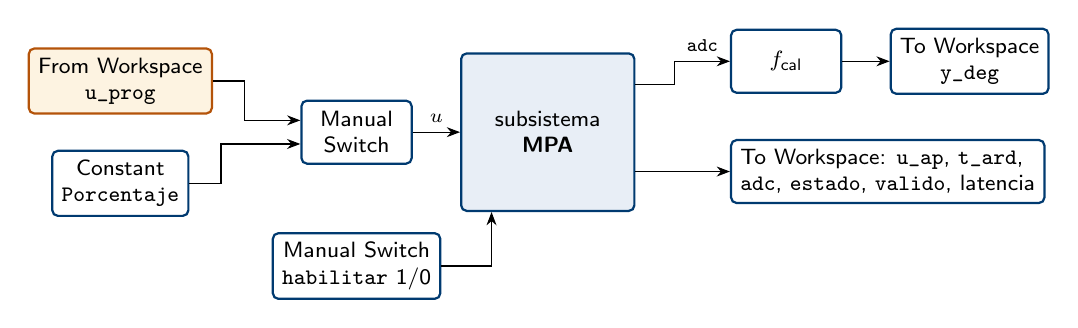
\begin{tikzpicture}[node distance=6mm]
  \node[blka] (prog) at (0,0.65) {From Workspace\\\sen{u_prog}};
  \node[blkw] (man) at (0,-0.65) {Constant\\\texttt{Porcentaje}};
  \node[blkw] (sw) at (3.0,0) {Manual\\Switch};
  \node[blk,right=of sw,minimum height=20mm,minimum width=22mm] (mpa) {subsistema\\\textbf{MPA}};
  \node[blkw] (hab) at (3.0,-1.7) {Manual Switch\\\texttt{habilitar} 1/0};
  \draw[->] (prog.east) -- ++(4mm,0) |- ($(sw.west)+(0,1.5mm)$);
  \draw[->] (man.east) -- ++(4mm,0) |- ($(sw.west)+(0,-1.5mm)$);
  \draw[->] (sw) -- node[above,sig]{$u$} ($(mpa.west)+(0,0)$);
  \draw[->] (hab.east) -| ($(mpa.south west)+(4mm,0)$);
  \node[blkw,right=12mm of mpa,yshift=9mm] (cal) {$f_\text{cal}$};
  \node[blkw,right=of cal] (tw1) {To Workspace\\\sen{y_deg}};
  \draw[->] ($(mpa.east)+(0,6mm)$) -- ++(5mm,0) |- node[pos=0.75,above,sig]{\sen{adc}} (cal);
  \draw[->] (cal) -- (tw1);
  \node[blkw,right=12mm of mpa,yshift=-5mm,align=left] (tw2) {To Workspace: \sen{u_ap}, \sen{t_ard},\\\sen{adc}, \sen{estado}, \sen{valido}, latencia};
  \draw[->] ($(mpa.east)+(0,-5mm)$) -- (tw2);
\end{tikzpicture}}
\caption{\texttt{MPA\_XX\_ensayos.slx}. El mando sale de un programa preparado en MATLAB o, con el \blq{Manual Switch}, de una constante para la primera prueba. \blq{From Workspace}: \emph{Interpolate data} desmarcado, \emph{Sample time} 0.02, \emph{Holding final value}. Todos los \blq{To Workspace} en formato \emph{Array} con \emph{Sample time} $-1$: cada variable queda en el workspace como un vector columna, con un valor cada 0.02~s.}\label{fig:modeloensayos}
\end{figure}

\subsection{El ensayo de escalera}

El mando sube por escalones desde un poco por debajo de $u_\text{mov}$ hasta $u_{85}$ y vuelve a bajar. Cada escalón dura $T_h=\SI{10}{s}$: unos 6~s para que la lámina se asiente y los últimos 3~s (\texttt{Tprom}) para promediar. Si al final del escalón la lámina todavía oscila, usen 15~s.

El ensayo usa dos guiones, como la identificación: \texttt{programa\_escalera.m} antes del \emph{Run} y \texttt{analisis\_escalera.m} después.

\needspace{12\baselineskip}
\begin{lstlisting}[caption={\texttt{programa\_escalera.m}: lo que se ajusta antes del \emph{Run}.}]
modulo = 4;                  % numero de SU MPA
modelo = 'MPA_04_ensayos';   % nombre del .slx (sin extension)
uini = 6;     % [%]  primer escalon: un poco por debajo de u_mov (primera prueba)
ufin = 90;    % [%]  ultimo escalon: u con la lamina cerca de 85 grados
du   = 6;     % [%]  tamano del escalon (4 si quieren mas detalle)
Th   = 10;    % [s]  duracion de cada escalon (15 s si la lamina sigue oscilando)
Tprom = 3;    % [s]  ventana final de cada escalon que se promedia (ya asentada)
Tarm = 20;    % [s]  u = 0 al inicio: ENCENDER LA FUENTE en estos segundos
\end{lstlisting}

\begin{enumerate}[leftmargin=14pt]
  \item \textbf{\texttt{programa\_escalera.m} (F5, antes del ensayo)}: borra los datos de una corrida anterior, arma el programa de mando \sen{u_prog} y, si el modelo está abierto, fija el \emph{Stop time} y deja el \blq{From Workspace} sin interpolar. Con \emph{Interpolate data} marcado los escalones se vuelven una rampa continua y la lámina nunca se asienta. Con los valores del ejemplo son 29 escalones, unos 5 minutos.
  \item \emph{Run} en Simulink con el \blq{Manual Switch} en el programa; enciendan la fuente durante los primeros 20~s (con $u=0$).
  \item \textbf{\texttt{analisis\_escalera.m} (F5, después del ensayo)}, con las variables del ensayo en el workspace:
  \begin{itemize}[leftmargin=12pt]
    \item revisa el enlace: \sen{diff(t_ard)}, la latencia y que el tiempo del Arduino avance igual que el de Simulink (si Simulink va más lento, cada paso consumió más de un paquete);
    \item avisa si el mando no fue constante dentro de los escalones;
    \item promedia los últimos \texttt{Tprom} segundos de cada escalón y avisa si la lámina no se había asentado;
    \item grafica el mapa subiendo y bajando, la ganancia local $K(u)$ y el ensayo en el tiempo;
    \item estima $u_\text{mov}$, la histéresis máxima y el $u$ para 30°, 45° y 60°;
    \item guarda todo en \texttt{mapa\_MPAxx\_fecha.mat}. \ficha
  \end{itemize}
\end{enumerate}

\begin{cuidado}[Nombres que el guion espera del modelo]
\blq{From Workspace}: \sen{u_prog}. \blq{To Workspace} (formato \emph{Array}): \sen{y_deg}, \sen{u_ap}, \sen{t_ard} y, si existe, \sen{latencia}. Si cambian un nombre en el modelo, cámbienlo también en el guion. El tiempo sale del \blq{To Workspace} \sen{t} del \blq{Clock} o de \sen{tout}; si no hay ninguno, el guion lo arma con el paso de 0.02~s. Si los datos duran menos que el ensayo programado, el guion se detiene: la corrida se cortó o las variables son de otra corrida.
\end{cuidado}

\subsection{Cómo se lee: el mapa de la MPA 4}

\begin{figure}[H]\centering
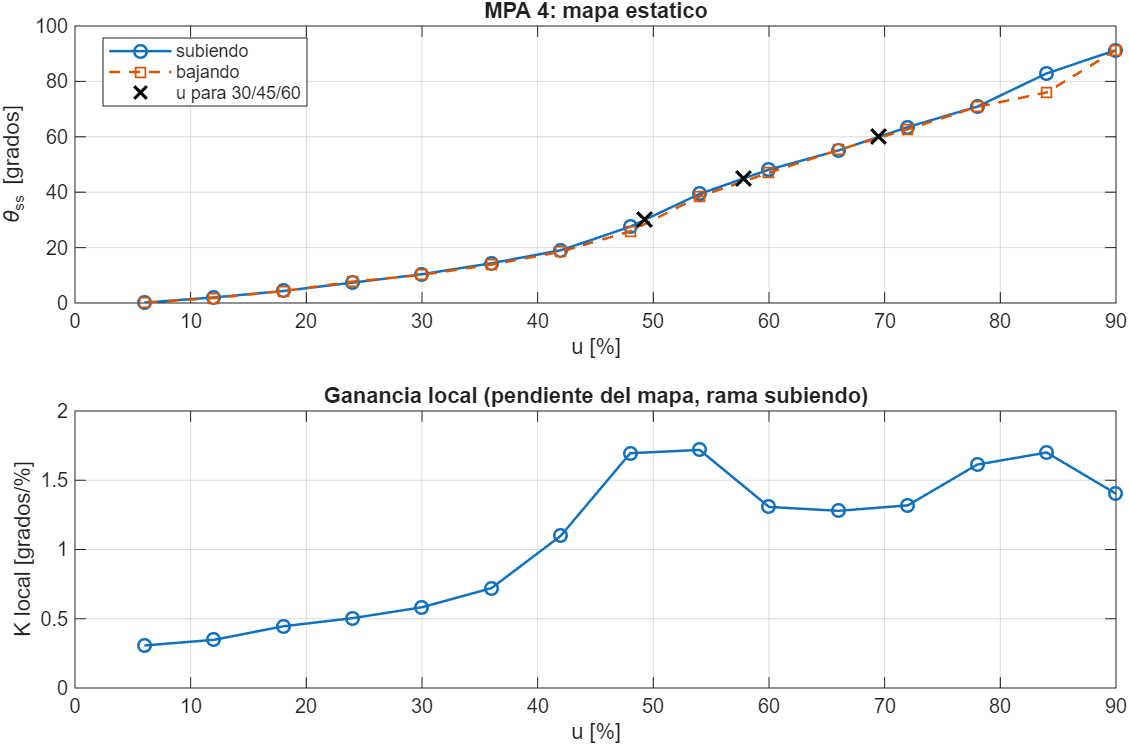
\includegraphics[width=0.88\linewidth]{figs/mapa_MPA04.png}
\caption{Mapa estático medido en la MPA~4 con \texttt{analisis\_escalera.m} (escalones de 6\,\%). Arriba: $\theta_{ss}$ subiendo y bajando, con el $u$ para 30°, 45° y 60°. Abajo: ganancia local $K(u)=d\theta_{ss}/du$ en la rama subiendo. Su MPA dará otros números, pero la forma debería parecerse.}\label{fig:mapa}
\end{figure}

\begin{nota}[Lo que dice este mapa de la planta]
\begin{itemize}[leftmargin=12pt]
  \item \textbf{La curva tiene tres zonas.}
  \begin{itemize}[leftmargin=10pt]
    \item Por debajo de $u\approx 42\,\%$ la lámina sube poco: $K$ va de 0.3 a 0.7~°/\%. El empuje de una hélice crece más o menos con el cuadrado de su velocidad, así que con poco mando cada punto adicional aporta poco empuje.
    \item Entre 48 y 75\,\% la curva es casi una recta, con $K\approx 1.3$--$1.7$~°/\%. Es la mejor zona para operar.
    \item Por encima de unos 78\,\% ($\theta>70°$) la lámina no se queda quieta: el chorro se vuelve turbulento, ahí están los escalones que no se asentaron y la única histéresis apreciable (unos 7° en 84\,\%). Esa zona no sirve como punto de operación.
  \end{itemize}
  \item \textbf{Histéresis casi nula hasta 78\,\%}: las dos ramas se superponen. La fricción del eje no pesa en el modelo, y al punto de operación se puede llegar desde cualquier lado.
  \item \textbf{Despegue}: con 6\,\% la lámina sigue en reposo; con 12\,\% ya se separó unos 2°.
  \item \textbf{Mando para 30°, 45° y 60°}: 49.2, 57.8 y 69.5\,\%. Van a la ficha.
\end{itemize}
\end{nota}

\begin{itemize}[leftmargin=12pt]
  \item \textbf{Punto de operación}: el reto asigna un ángulo $\theta_0$ lejos de los dos topes. Del mapa sale el $u_0$ que lo produce. En la MPA~4, el tramo recto entre 45° y 60° ($u_0$ de 58 a 70\,\%, $K\approx1.3$) es el más cómodo: ahí un escalón de 4\,\% mueve la lámina unos 5°, justo lo que pide la identificación.
  \item \textbf{El modelo lineal vale solo cerca de $u_0$}: entre 15° y 50° la ganancia local casi se duplica, y $B$ es proporcional a $K$. Un controlador diseñado en un punto ve otra planta en el otro: puede quedar lento en uno y oscilar en el otro. Para recorrer toda la carrera hace falta cambiar las ganancias según el punto (\emph{gain scheduling}).
  \item \textbf{Ganancia local}: la pendiente en $u_0$, $K_\text{mapa}\approx\big(\theta_{ss}(u_0+\Delta)-\theta_{ss}(u_0-\Delta)\big)/(2\Delta)$ [°/\%]. Compárenla con la del escalón de la sección~\ref{sec:escalones}; si difieren más del 25\,\%, algo está mal en uno de los dos ensayos.
  \item \textbf{Histéresis}: si en su MPA subiendo y bajando difieren más de 3° en el mismo $u$, lleguen siempre al punto de operación desde el mismo lado y díganlo en el reporte.
\end{itemize}

% =====================================================================
\section{Identificación para espacio de estados}\label{sec:ident}

\subsection{La estructura del modelo}

Dividiendo~\eqref{eq:lineal} por $J$ queda un sistema de segundo orden,
\begin{equation}
\ddot{\tilde\theta} + 2\zeta\omega_n\,\dot{\tilde\theta} + \omega_n^2\,\tilde\theta = K\omega_n^2\,\tilde u,
\qquad
\omega_n^2=\frac{k}{J},\quad 2\zeta\omega_n=\frac{b}{J},\quad K=\frac{\kappa}{k}\ [\text{°/\%}].
\label{eq:segundo}
\end{equation}
Con estados físicos, $x_1=\tilde\theta$ (ángulo) y $x_2=\dot{\tilde\theta}$ (velocidad angular):
\begin{equation}
\dot x=\underbrace{\begin{bmatrix}0 & 1\\ -\omega_n^2 & -2\zeta\omega_n\end{bmatrix}}_{A}x
+\underbrace{\begin{bmatrix}0\\ K\omega_n^2\end{bmatrix}}_{B}\tilde u,
\qquad
\tilde y=\underbrace{\begin{bmatrix}1 & 0\end{bmatrix}}_{C}x,\qquad D=0.
\label{eq:ss}
\end{equation}
Las unidades: $x_1$ en °, $x_2$ en °/s, $B$ en °/(\%·s²). Todo el modelo cabe en \textbf{tres números por punto de operación}: $\omega_n$, $\zeta$ y $K$. Los valores propios de $A$ son $-\sigma\pm j\omega_d$, con $\sigma=\zeta\omega_n$ y $\omega_d=\omega_n\sqrt{1-\zeta^2}$.

\begin{nota}[La idea: un ensayo para cada matriz]
\begin{itemize}[leftmargin=12pt]
  \item \textbf{$A$ sale de la lámina sola.} Se aplica un pulso corto de mando; cuando termina, el mando queda constante en $u_0$ y la lámina oscila libre alrededor de $\theta_0$. Esa \emph{respuesta libre} depende solo de $A$: la separación entre picos da $\omega_d$ y la envolvente da $\sigma$. Son los polos, medidos directamente.
  \item \textbf{$B$ sale del motor.} Un escalón pequeño $\Delta u$ lleva la lámina a otro equilibrio: $K=\Delta\theta_{ss}/\Delta u$, y con eso $B$.
  \item \textbf{$C$ ya se conoce}: se mide el ángulo y no la velocidad.
\end{itemize}
\end{nota}

\subsection{El ensayo programado}

Todo sale de \textbf{una corrida de unos 5 minutos} con el modelo de la figura~\ref{fig:modeloensayos}: armado, llegada al punto de operación, tres pulsos (para promediar $A$), un escalón hacia arriba (para estimar $K$) y uno hacia abajo (para \emph{validar}, sin usarlo para estimar).

\begin{figure}[H]\centering
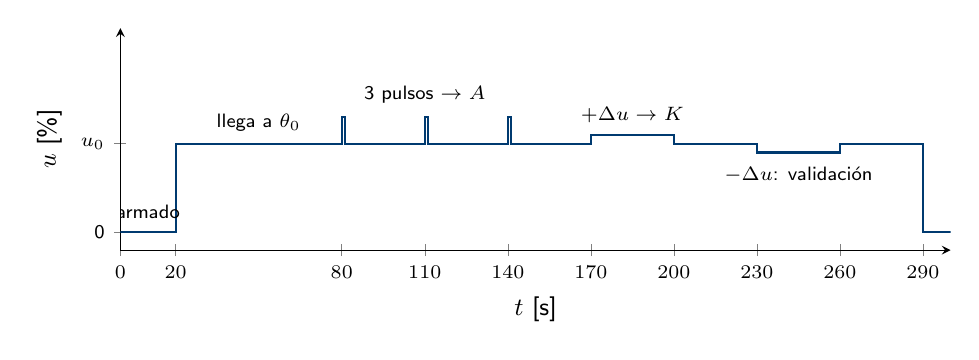
\begin{tikzpicture}
\begin{axis}[width=\linewidth,height=4.4cm,xmin=0,xmax=300,ymin=-8,ymax=92,
  xlabel={$t$ [s]},ylabel={$u$ [\%]},axis lines=left,
  tick label style={font=\scriptsize},label style={font=\small},
  xtick={0,20,80,110,140,170,200,230,260,290},ytick={0,40},yticklabels={0,$u_0$}]
  \addplot[azulEIA,thick,const plot] coordinates {(0,0) (20,40) (80,52) (81.2,40) (110,52) (111.2,40) (140,52) (141.2,40) (170,44) (200,40) (230,36) (260,40) (290,0) (300,0)};
  \node[font=\scriptsize,anchor=south] at (axis cs:10,2) {armado};
  \node[font=\scriptsize,anchor=south] at (axis cs:50,41) {llega a $\theta_0$};
  \node[font=\scriptsize,anchor=south] at (axis cs:110,54) {3 pulsos $\to A$};
  \node[font=\scriptsize,anchor=south] at (axis cs:185,45) {$+\Delta u\to K$};
  \node[font=\scriptsize,anchor=north] at (axis cs:245,34) {$-\Delta u$: validación};
\end{axis}
\end{tikzpicture}
\caption{Forma del programa (el ancho de los pulsos está exagerado para que se vean). El firmware redondea los bordes con su rampa.}\label{fig:programa}
\end{figure}

\needspace{20\baselineskip}
\begin{lstlisting}[caption={Programa del ensayo de identificación (\texttt{programa\_identificacion.m}).}]
modulo = 4;   %      numero de SU MPA
u0   = 40;    % [%]  mando del punto de operacion (del mapa estatico)
Ap   = 10;    % [%]  amplitud del pulso
tp   = 0.4;   % [s]  duracion del pulso
dU   = 4;     % [%]  escalon pequeno
Tarm = 20;    % [s]  u = 0 para armar el ESC (encender la fuente aqui)
Tesp = 30;    % [s]  espera entre eventos
rampa = 50;   % [%/s] RAMPA_PCT_S del firmware
ev = [0 0; Tarm u0];
t  = Tarm + 2*Tesp;                          % 60 s para asentarse en theta0
tPul = zeros(1,3);
for k = 1:3
    tPul(k) = t;
    ev = [ev; t u0+Ap; t+tp u0];   t = t + Tesp;
end
tSub = t;  ev = [ev; t u0+dU];   t = t + Tesp;   % escalon arriba (estimacion)
           ev = [ev; t u0];      t = t + Tesp;   % regreso
tBaj = t;  ev = [ev; t u0-dU];   t = t + Tesp;   % escalon abajo (validacion)
           ev = [ev; t u0];      t = t + Tesp;
ev = [ev; t 0];                                  % fin: motor a cero
u_prog = timeseries(ev(:,2), ev(:,1));
Tfin = t + 5;                                    % Stop time
\end{lstlisting}

\begin{cuidado}[Cómo escoger $A_p$, $t_p$ y $\Delta u$]
\begin{itemize}[leftmargin=12pt]
  \item El pulso debe sacar la lámina entre \textbf{8° y 15°} en el primer pico. Con la rampa, un pulso de $A_p=10\,\%$ tarda \SI{0.2}{s} en subir y \SI{0.2}{s} en bajar: $t_p$ debe ser mayor que $A_p/50$~s.
  \item El escalón $\Delta u$ debe mover el equilibrio entre \textbf{5° y 8°}: $\Delta u\approx 6/K_\text{mapa}$. Con 4\,\% la rampa tarda \SI{0.08}{s}: despreciable frente a la lámina.
  \item Si al llegar el siguiente evento la lámina todavía oscila, aumenten \texttt{Tesp}.
\end{itemize}
\end{cuidado}

Después de la corrida comprueben la latencia y \sen{diff(t_ard)}. Las variables de los \blq{To Workspace} se sobrescriben en el siguiente \emph{Run}; por eso \texttt{analisis\_pulsos.m} guarda primero la corrida completa (\sen{y_deg}, \sen{u_ap}, \sen{t_ard} y el programa del ensayo) en \texttt{ident\_MPAxx\_fecha.mat}. Para retomar otro día basta con \texttt{load} de ese archivo.

\subsection{La matriz \texorpdfstring{$A$}{A}: respuesta libre después del pulso}\label{sec:pulsos}

Cuando termina la rampa de bajada del pulso ($t_\text{pulso}+t_p+A_p/50$), el mando queda fijo en $u_0$ y la lámina se mueve sola. Con $\tilde u=0$, la solución de~\eqref{eq:segundo} es una cosenoide amortiguada que depende solo de $A$:
\begin{equation}
\tilde\theta(t) = A_m\,e^{-\sigma t}\cos(\omega_d t+\varphi) + c,
\qquad
\omega_n=\sqrt{\sigma^2+\omega_d^2},
\qquad
\zeta=\frac{\sigma}{\omega_n}.
\label{eq:decremento}
\end{equation}
\texttt{analisis\_pulsos.m} ajusta los cinco parámetros ($A_m$, $\sigma$, $\omega_d$, $\varphi$ y un pequeño desfase $c$) a \textbf{todos} los puntos de los 6~s de respuesta libre, con \texttt{fminsearch} y varios valores iniciales de $\omega_d$. Así no depende de cuántos picos se alcancen a ver: en la MPA~4, con $\zeta\approx0.3$, la lámina da solo dos extremos por encima del ruido.

\begin{figure}[H]\centering
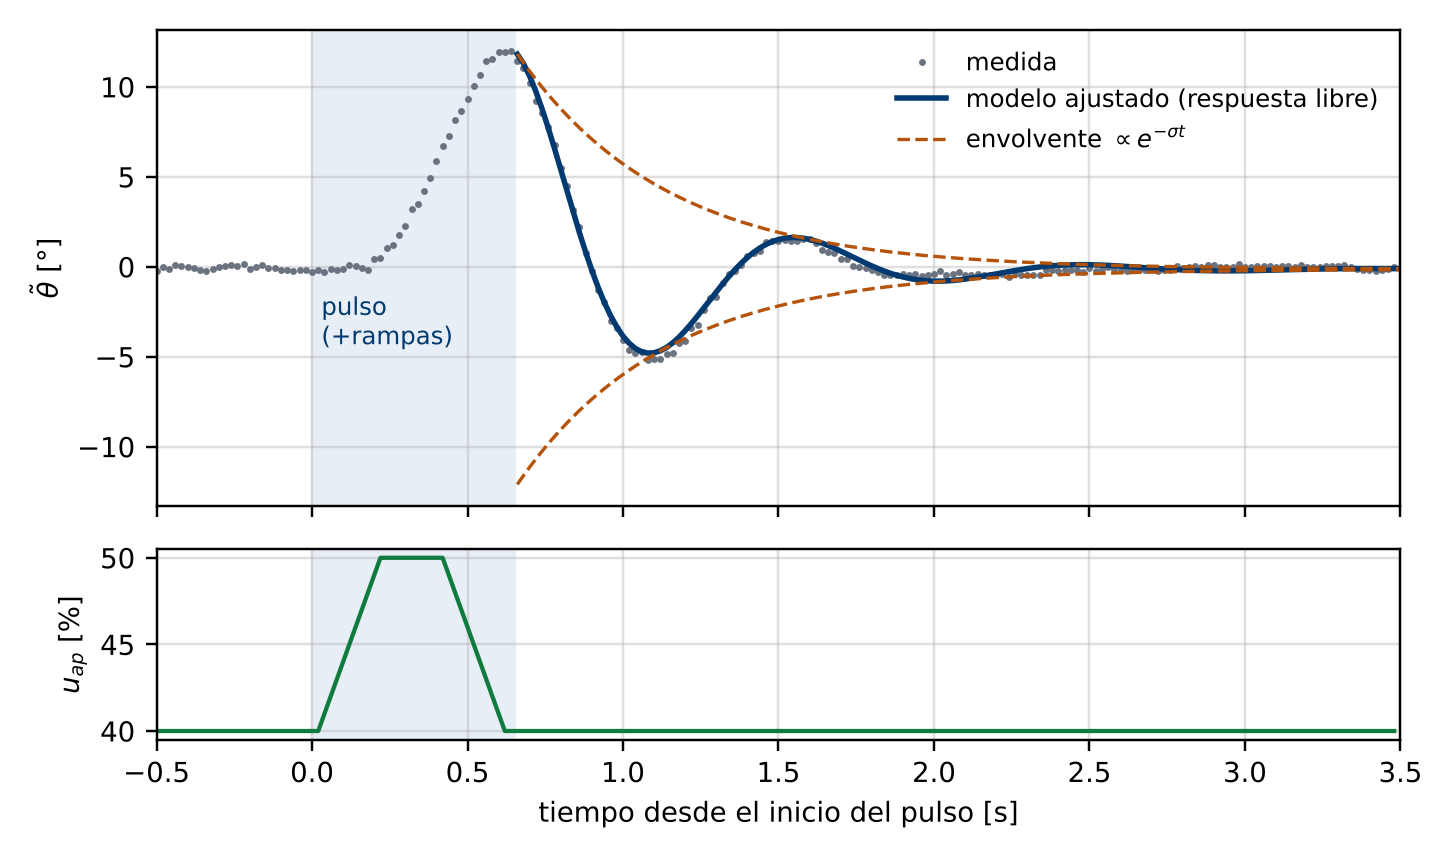
\includegraphics[width=0.86\linewidth]{figs/pulso_MPA04.png}
\caption{Primer pulso del ensayo de la MPA~4 ($u_0=40\,\%$, $\theta_0\approx17°$, $A_p=10\,\%$, $t_p=0.4$~s). El modelo~\eqref{eq:decremento} se ajusta desde que termina la rampa de bajada: $\sigma=2.10$~s$^{-1}$, $\omega_d=6.78$~rad/s, es decir $\omega_n=7.10$~rad/s y $\zeta=0.30$. Note el retardo: la lámina empieza a moverse unos 0.1~s después del mando.}\label{fig:libre}
\end{figure}

\begin{nota}[Lectura a ojo, para comprobar el ajuste]
Dos extremos sucesivos están separados medio periodo, $\pi/\omega_d$, y su cociente es $e^{-\sigma\pi/\omega_d}$. En la figura~\ref{fig:libre}: mínimo de $-4.9°$ en 1.08~s y máximo de $+1.6°$ en 1.55~s. Entonces $\omega_d\approx\pi/0.47\approx6.7$~rad/s y $\sigma\approx\ln(4.9/1.6)/0.47\approx2.4$~s$^{-1}$, cerca del ajuste. Con solo dos extremos la lectura a ojo es frágil; el ajuste usa los 300 puntos.
\end{nota}

\needspace{20\baselineskip}
\begin{lstlisting}[caption={Núcleo de \texttt{analisis\_pulsos.m} (extracto; el archivo también grafica y avisa).}]
Tlib = 6;                                    % [s] de respuesta libre
opc  = optimset('Display', 'off', 'MaxFunEvals', 5000, 'MaxIter', 5000);
for k = 1:numel(tPul)
    y0 = mean(y(t >= tPul(k)-5 & t < tPul(k)));      % equilibrio antes del pulso
    tl = tPul(k) + tp + Ap/rampa + 0.05;             % termino la rampa de bajada
    w  = t >= tl & t < tl + Tlib;                    % respuesta libre
    tt = t(w) - tl;   z = y(w) - y0;
    libre = @(p) p(1)*exp(-p(2)*tt).*cos(p(3)*tt + p(4)) + p(5);
    J     = @(p) sum((z - libre(p)).^2);
    Jmin = inf;
    for wd0 = [3 5 7 9 12]                           % varios arranques en wd
        [p, Jp] = fminsearch(J, [z(1) 2 wd0 0 0], opc);
        if Jp < Jmin, Jmin = Jp; pb = p; end
    end
    res(k,:) = [pb(2), abs(pb(3)), 100*(1 - sqrt(Jmin)/norm(z - mean(z))), max(abs(z))];
end
sigma = mean(res(:,1));  wd = mean(res(:,2));
wn = hypot(sigma, wd);   zeta = sigma/wn;
\end{lstlisting}

\begin{nota}[Cuándo creerle al resultado]
Los tres pulsos deben dar $\omega_n$ dentro de $\pm10\,\%$ y $\zeta$ dentro de $\pm25\,\%$ entre sí, y cada ajuste un \emph{fit} por encima del 70\,\%. En la MPA~4 dieron $\omega_n=7.10$, 6.15 y 6.17~rad/s y $\zeta=0.30$, 0.35 y 0.32, con \emph{fit} de 88--89\,\%: promedio $\omega_n=6.47$~rad/s, $\zeta=0.32$. Si un pulso se sale, miren su gráfica: un golpe contra el tope, una racha del chorro o un pulso que no alcanzó a asentarse lo explican casi siempre.
\end{nota}

\subsection{La matriz \texorpdfstring{$B$}{B}: los escalones}\label{sec:escalones}

\needspace{8\baselineskip}
\begin{lstlisting}[caption={Ganancia estática con el escalón de subida (\texttt{analisis\_escalones\_modelo.m}, parte 1).}]
ym  = @(a,b) mean(y(t >= a & t < b));                       % promedio en [a, b)
Ksub = (ym(tSub+Tesp-5, tSub+Tesp) - ym(tSub-5, tSub)) / dU;
Kbaj = (ym(tBaj+Tesp-5, tBaj+Tesp) - ym(tBaj-5, tBaj)) / (-dU);
fprintf('K subiendo = %.3f   K bajando = %.3f  grados/%%\n', Ksub, Kbaj)
\end{lstlisting}

Si $K_\text{sub}$ y $K_\text{baj}$ difieren más del 15\,\%, el escalón es demasiado grande para la curvatura del mapa en ese punto, o la histéresis está pesando: repitan con $\Delta u$ menor.

\subsection{Las matrices, el retardo y la validación}

\needspace{20\baselineskip}
\begin{lstlisting}[caption={Modelo en espacio de estados y validación con el escalón de bajada (parte 2).}]
K = Ksub;
A = [0 1; -wn^2 -2*zeta*wn];   B = [0; K*wn^2];   C = [1 0];   D = 0;
G = ss(A, B, C, D, 'StateName', {'theta','omega'}, 'StateUnit', {'grados','grados/s'}, ...
       'InputName', 'u', 'InputUnit', '%', 'OutputName', 'theta', 'OutputUnit', 'grados');
% --- datos de validacion: escalon de bajada, en desviacion (u aplicado de verdad)
u  = double(u_ap(:));
w  = t >= tBaj-5 & t < tBaj+Tesp;
tv = t(w) - t(find(w,1));
dy = y(w) - ym(tBaj-5, tBaj);    du = u(w) - u0;
% --- retardo: el que mejor alinea modelo y medida
dl = 0:Ts:0.3;   J = zeros(size(dl));
for i = 1:numel(dl)
    G.InputDelay = dl(i);   J(i) = norm(dy - lsim(G, du, tv));
end
[~, ib] = min(J);  retardo = dl(ib);  G.InputDelay = retardo;
ys  = lsim(G, du, tv);
fit = 100*(1 - norm(dy - ys)/norm(dy - mean(dy)));
plot(tv, dy, tv, ys, '--', 'LineWidth', 1.2); grid on
legend('medido', 'modelo'); xlabel('t [s]'); ylabel('\Delta\theta [grados]')
fprintf('retardo = %.2f s   fit de validacion = %.0f %%\n', retardo, fit)
save(sprintf('MPA%02d_modelo_%s.mat', modulo, datestr(now,'yyyymmdd')), ...
     'A','B','C','D','wn','zeta','K','u0','retardo','fit')
\end{lstlisting}

El retardo que aparece junta el viaje por el USB, el pulso de \SI{20}{ms} y la dinámica del motor que el modelo de segundo orden deja por fuera. \textbf{No va en las matrices}: queda anotado y entra al lazo simulado, porque es lo que puede volver oscilante un diseño demasiado rápido. La validación usa \sen{u_ap}, el mando que de verdad aplicó el Arduino.

\begin{figure}[H]\centering
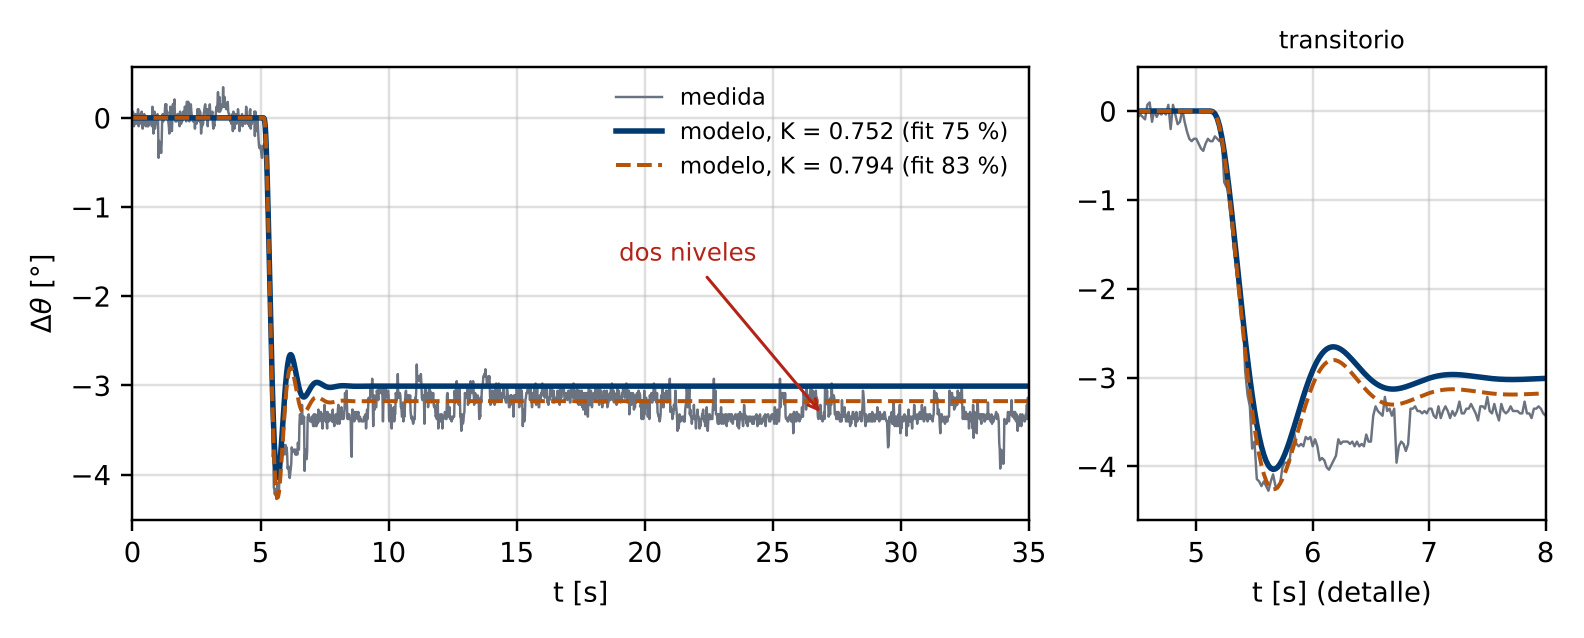
\includegraphics[width=\linewidth]{figs/validacion_MPA04.png}
\caption{Validación con el escalón de bajada en la MPA~4 ($u_0=40\,\%$, $\Delta u=-4\,\%$), que no se usó para estimar. Modelo de los pulsos ($\omega_n=6.47$~rad/s, $\zeta=0.32$) con retardo de 0.10~s. Continua: $K$ del escalón de subida; discontinua: promedio de subida y bajada.}\label{fig:validacion}
\end{figure}

\begin{nota}[Lo que dice esta validación]
\begin{itemize}[leftmargin=12pt]
  \item \textbf{La caída se reproduce bien}: el instante en que arranca (retardo), la pendiente y el primer mínimo coinciden. Esa es la parte que gobierna un lazo cerrado.
  \item \textbf{El nivel final difiere unos 0.3°}: bajando, la planta respondió con $K=0.837$ y subiendo con 0.752, un 11\,\% menos. Es la curvatura del mapa estático alrededor de $u_0$. Con el promedio, 0.794, el \emph{fit} pasa de 75 a 83\,\%. La acción integral del Reto~3 elimina ese error en estado estacionario, pero el diseño debe tolerarlo.
  \item \textbf{Bajando, la lámina se amortigua más}: después del mínimo casi no rebota, y el modelo sí. La planta no es simétrica.
  \item \textbf{La medida salta entre dos niveles}, unos $-3.1°$ y $-3.35°$, y se queda un rato en cada uno: no es ruido blanco. Puede ser el chorro alternando entre dos patrones de flujo o la resolución del potenciómetro (unos 0.25° por cuenta). Ningún modelo lineal lo reproduce; para el control es una perturbación.
\end{itemize}
\end{nota}

\begin{tcolorbox}[enhanced,colback=azulClaro,colframe=azulEIA,boxrule=0.6pt,title={Modelo de la MPA 4 en $\theta_0\approx17.4°$, $u_0=40\,\%$},fonttitle=\bfseries\small,coltitle=white,colbacktitle=azulEIA]
\small
\[
A=\begin{bmatrix}0 & 1\\ -41.9 & -4.15\end{bmatrix},\qquad
B=\begin{bmatrix}0\\ 31.5\end{bmatrix},\qquad
C=\begin{bmatrix}1 & 0\end{bmatrix},\qquad
\lambda(A)=-2.08\pm6.13j,\qquad T_d\approx0.10~\text{s}.
\]
Con $\omega_n=6.47$~rad/s, $\zeta=0.32$ y $K=0.752$~°/\% (escalón de subida). Es el ejemplo de este manual; cada equipo identifica su MPA en su propio punto de operación.
\end{tcolorbox}

\begin{nota}[Preguntas de validación (no hay un \emph{fit} mágico)]
\begin{itemize}[leftmargin=12pt]
  \item ¿El modelo reproduce el escalón de bajada, que no se usó para estimar: sentido, valor final ($\pm15\,\%$), número de oscilaciones visibles y periodo?
  \item ¿$K$ del escalón y $K_\text{mapa}$ de la escalera concuerdan ($\pm25\,\%$)?
  \item ¿El periodo de las oscilaciones del escalón coincide con el $\omega_d$ de los pulsos?
  \item ¿El modelo se identificó en el mismo punto de operación donde se va a controlar?
\end{itemize}
Con eso, anoten $\omega_n$, $\zeta$, $K$, el retardo, $u_0$ y $\theta_0$. \ficha
\end{nota}

\subsection{Otra vía: el escalón con \texttt{ident} (opcional)}\label{sec:noosc}

\begin{nota}[El mismo modelo con lo que vieron en Modelos y Simulación]
El escalón de subida, recortado y trasladado al origen, se puede llevar a \texttt{ident} con un \emph{Process Model} de 2 polos subamortiguado con retardo (P2DU). Da $K$, $\omega_n$, $\zeta$ y $T_d$ de una vez, y con ellos se arman $A$, $B$ y $C$ con~\eqref{eq:ss}. En la MPA~4 dio $K=0.82$~°/\%, $\omega_n=5.9$~rad/s, $\zeta=0.28$ y $T_d=0.08$~s, en línea con los pulsos ($\omega_n=6.47$, $\zeta=0.32$). Que dos ensayos distintos den los mismos polos es la mejor prueba de que el modelo es creíble. Es también el camino si la lámina casi no oscila después del pulso.
\end{nota}


Si la respuesta libre casi no se separa del ruido (lámina muy amortiguada) o el ajuste da un \emph{fit} bajo, primero intenten un pulso un poco mayor, sin pasar de 15°. Por línea de comandos, el equivalente de \texttt{ident} es:

\needspace{8\baselineskip}
\begin{lstlisting}[caption={Alternativa: dos polos, sin ceros, con retardo estimado.}]
w   = t >= tSub-5 & t < tSub+Tesp;
dat = iddata(y(w) - ym(tSub-5,tSub), u(w) - u0, Ts);
G2  = tfest(dat, 2, 0, NaN);            % 2 polos, 0 ceros, retardo libre
[num, den] = tfdata(G2, 'v');           % den = [1  2*zeta*wn  wn^2]
wn = sqrt(den(3));  zeta = den(2)/(2*wn);  K = num(end)/den(3);
\end{lstlisting}

Las matrices se arman igual con~\eqref{eq:ss}. No usen la realización que entrega el toolbox (\texttt{ss(G2)} o \texttt{idss}) sin mirarla: sus estados no son ángulo y velocidad, y el Reto 3 los necesita con significado físico.

\subsection{Lo que el modelo deja por fuera}\label{sec:nomodela}

\begin{table}[H]\centering\small
\caption{Hipótesis del modelo y dónde se notan.}\label{tab:hipotesis}
\rowcolors{2}{azulClaro}{white}
\begin{tabularx}{\linewidth}{@{}>{\raggedright\arraybackslash}p{3.9cm} >{\raggedright\arraybackslash}X@{}}\toprule
\textbf{Lo que se ignora} & \textbf{Dónde aparece}\\\midrule
Dinámica del motor y la hélice ($\tau_m$) & Como retardo aparente en el escalón. Es el tercer estado que no se modela.\\
Retardo del USB y del pulso de \SI{20}{ms} & Igual que el anterior: se mide junto.\\
No linealidad de la planta & $K$, $\omega_n$ y $\zeta$ cambian con $\theta_0$. El modelo vale cerca de su punto.\\
Rampa del firmware & Limitador de rapidez de $\pm50$\,\%/s. Inactivo en señal pequeña; activo en cambios grandes de referencia.\\
Zona muerta, saturación y tope & El mando útil está en $[u_\text{arr},\,100]$; por debajo de $u_\text{mov}$ la lámina descansa en el tope.\\
Empuje en un solo sentido & La hélice solo empuja hacia arriba; hacia abajo actúa la gravedad.\\
Cuantización del sensor & Del orden de 0.2°/cuenta (menos con el promedio de 16). Al derivar $y$ con $T_s=\SI{0.02}{s}$, una sola cuenta equivale a unos \textbf{10°/s} de «velocidad»: la velocidad angular no se mide, se estima.\\
Turbulencia del chorro & Pequeñas oscilaciones irregulares sobre el equilibrio que ningún modelo lineal reproduce.\\\bottomrule
\end{tabularx}
\end{table}

\subsection{Otro punto de operación (si el reto lo pide)}

Repitan el ensayo programado con otro $\theta_0$ (por ejemplo 30° y 60°). Comparar $\omega_n$, $\zeta$ y $K$ entre los dos puntos muestra, con números, cuánto cambia la planta, y es la base de la programación de ganancias (\emph{gain scheduling}).

% =====================================================================
\section{Preparar el lazo cerrado}\label{sec:lazo}

El controlador y el observador se diseñan en el Reto 3. Este manual deja lista la \textbf{interfaz}: cómo entran y salen las señales, en qué unidades y qué se registra.

\begin{figure}[H]\centering
\resizebox{\linewidth}{!}{%
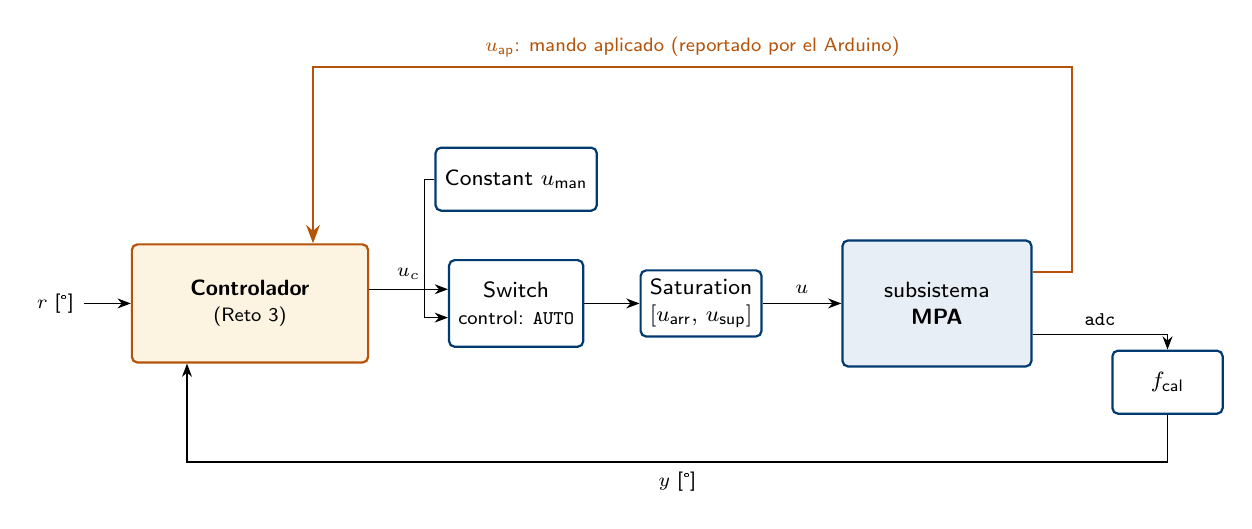
\begin{tikzpicture}[node distance=7mm]
  \node[sig] (r) {$r$ [°]};
  \node[blka,right=6mm of r,minimum width=30mm,minimum height=15mm] (ctl) {\textbf{Controlador}\\\scriptsize (Reto 3)};
  \node[blkw,right=10mm of ctl,minimum height=11mm] (ma) {Switch\\\scriptsize control: \texttt{AUTO}};
  \node[blkw,above=6mm of ma] (uman) {Constant $u_\text{man}$};
  \node[blkw,right=of ma] (sat) {Saturation\\$[u_\text{arr},\,u_\text{sup}]$};
  \node[blk,right=10mm of sat,minimum height=16mm,minimum width=24mm] (mpa) {subsistema\\\textbf{MPA}};
  \node[blkw,right=10mm of mpa,yshift=-10mm] (cal) {$f_\text{cal}$};
  \draw[->] (r) -- (ctl);
  \draw[->] ($(ctl.east)+(0,1.8mm)$) -- node[above,sig]{$u_c$} ($(ma.west)+(0,1.8mm)$);
  \draw[->] (uman) -| ($(ma.west)+(-3mm,-1.8mm)$) -- ($(ma.west)+(0,-1.8mm)$);
  \draw[->] (ma) -- (sat); \draw[->] (sat) -- node[above,sig]{$u$} (mpa);
  \draw[->] ($(mpa.east)+(0,-4mm)$) -| node[pos=0.25,above,sig]{\sen{adc}} (cal.north);
  \draw[->] (cal.south) |- ++(0,-6mm) -| node[pos=0.25,below,sig]{$y$ [°]} ($(ctl.south)+(-8mm,0)$);
  \draw[->,ambar,thick] ($(mpa.east)+(0,4mm)$) -- ++(5mm,0) |- ++(0,26mm) -| node[pos=0.25,above,sig,ambar]{$u_\text{ap}$: mando aplicado (reportado por el Arduino)} ($(ctl.north)+(8mm,0)$);
\end{tikzpicture}}
\caption{Interfaz de \texttt{MPA\_XX\_lazo.slx}. Todo lo que está fuera de la caja ámbar queda fijo. $u_\text{ap}$ viene del Arduino: ya incluye la rampa, el tope y el estado SEGURO.}\label{fig:lazo}
\end{figure}

\begin{itemize}[leftmargin=12pt]
  \item \textbf{Unidades absolutas afuera, desviaciones adentro.} La caja recibe $r$ e $y$ en grados y $u_\text{ap}$ en \%, y entrega $u_c$ en \%. Si el diseño trabaja en desviación, la caja resta $\theta_0$ y $u_0$ al entrar y suma $u_0$ al salir.
  \item \textbf{La caja recibe el mando aplicado.} El controlador del Reto 3 tiene estados internos, y esos estados necesitan saber qué recibió de verdad la planta: en manual no es $u_c$; cuando el mando satura o la rampa lo frena, tampoco. Es la misma idea del seguimiento del Reto 2, y aquí la señal la mide el propio Arduino.
  \item \textbf{La saturación usa los límites de la ficha}, $[u_\text{arr},u_\text{sup}]$.
  \item \textbf{El arranque no cambia}: MAN con $u_\text{man}=0$, fuente encendida, armado, $u_\text{man}=u_0$, esperar a que la lámina se asiente en $\theta_0$, y solo entonces AUTO.
  \item \textbf{Registro}: $r$, $y$, $u_c$, $u_\text{ap}$, \texttt{AUTO}, \sen{t_ard} y la latencia, con \blq{To Workspace} a $T_s$.
  \item \textbf{Lazo simulado en paralelo}: \blq{Saturation} y \blq{Rate Limiter} ($\pm50$\,\%/s) seguidos de un \blq{State-Space} con las matrices identificadas y el retardo, alimentado con $u-u_0$ y con $\theta_0$ sumado a su salida. Arranca en equilibrio y permite comparar planta y modelo con los mismos mandos.
\end{itemize}

% =====================================================================
\section{Problemas frecuentes}

\begin{table}[H]\centering\small
\caption{Síntoma, comprobación y acción.}\label{tab:problemas}
\rowcolors{2}{azulClaro}{white}
\begin{tabularx}{\linewidth}{@{}>{\raggedright\arraybackslash}p{3.7cm} >{\raggedright\arraybackslash}p{4.7cm} >{\raggedright\arraybackslash}X@{}}\toprule
\textbf{Síntoma} & \textbf{Comprueben} & \textbf{Acción}\\\midrule
Simulink se queda esperando y sale un \emph{timeout} & Puerto COM, monitor serie del IDE abierto, firmware cargado & Cierren el IDE, revisen el COM; si alguien usó Connected IO, vuelvan a cargar el firmware.\\
Error de tamaños en una MATLAB Function & Se pegó el código completo, con sus funciones auxiliares & Peguen el archivo entero; \emph{Data type} del \blq{Serial Receive} en \texttt{uint8}.\\
\sen{valido} en 0, \sen{n_malos} sube & Versiones distintas de firmware y funciones & Firmware v2 con los \texttt{.m} de la misma versión.\\
El ESC pita y no arma & ¿La fuente se encendió con el modelo corriendo en $u=0$? Señal en pin 6 y tierra común & Apaguen la fuente, 5~s, enciendan con el modelo en cero.\\
\sen{estado} en 0 y el motor no arranca & ¿Se arrancó con $u\ne0$? ¿\texttt{habilitar} en 0? & Lleven $u$ a 0 (rearme) y \texttt{habilitar} a 1.\\
El motor gira pero la lámina casi no sube & Hélice volteada o giro al revés & Sección~\ref{sec:helice}: orientación y, si hace falta, intercambiar dos fases.\\
La fuente se protege (se apaga) & Cambios bruscos, \texttt{RAMPA\_PCT\_S} en 0 & Desconecten la fuente de la red unos segundos; mantengan la rampa.\\
Ángulo incorrecto & Calibración de este módulo & Comprueben tres marcas con el motor apagado; recalibren.\\
Latencia mayor que 1 & Scopes o Displays abiertos, otros programas & Cierren ventanas; registren con \blq{To Workspace}.\\
El ensayo tarda el doble; \sen{diff(t_ard)} da 0.04 y \sen{diff(seq)} da 2 & \emph{Block sample time} del \blq{Serial Receive} y \emph{Fixed-step size} del modelo & Los dos en 0.02. Con 0.01, Simulink lee dos paquetes por paso y su tiempo avanza a la mitad del real: el mapa estático no cambia, pero la identificación da $\omega_n$ a la mitad.\\
Ajuste del pulso con \emph{fit} bajo o $\omega_n$ dispersa & Gráfica de cada pulso: tamaño del primer pico, golpes, rachas & Pulso algo mayor ($A_p$ o $t_p$); si no, sección~\ref{sec:noosc}.\\
$K$ subiendo $\ne$ $K$ bajando & Tamaño de $\Delta u$, histéresis & Reduzcan $\Delta u$; lleguen al punto desde el mismo lado.\\\bottomrule
\end{tabularx}
\end{table}

% =====================================================================
\section{Lista de comprobación}

\begin{tcolorbox}[enhanced,colback=white,colframe=verdeOK,boxrule=0.6pt,sharp corners=south,title=Antes de encender la fuente,fonttitle=\bfseries\small,coltitle=white,colbacktitle=verdeOK]
\small
$\square$ Módulo identificado y ficha a la mano. \quad $\square$ Firmware v2 cargado; monitor serie cerrado.\\
$\square$ COM correcto en los tres bloques seriales. \quad $\square$ Calibración de \emph{este} módulo cargada.\\
$\square$ $u=0$ y \texttt{habilitar} $=1$. \quad $\square$ Simulink corriendo: \sen{estado} $=1$, \sen{valido} $=1$, latencia 0--1.\\
$\square$ Hélice orientada y sentido del aire comprobado. \quad $\square$ Manos lejos de la hélice.
\end{tcolorbox}

\begin{tcolorbox}[enhanced,colback=white,colframe=azulEIA,boxrule=0.6pt,sharp corners=south,title=Antes de aceptar un modelo,fonttitle=\bfseries\small,coltitle=white,colbacktitle=azulEIA]
\small
$\square$ \sen{diff(t_ard)} $=0.02$ y latencia 0--1 en todo el ensayo. \quad $\square$ Lámina sin tocar topes.\\
$\square$ Tres pulsos coherentes ($\omega_n$ $\pm10\,\%$, $\zeta$ $\pm25\,\%$). \quad $\square$ $K_\text{sub}$ y $K_\text{baj}$ dentro del 15\,\%.\\
$\square$ $K$ del escalón y del mapa dentro del 25\,\%. \quad $\square$ Validación con el escalón de bajada.\\
$\square$ Matrices con estados físicos y unidades. \quad $\square$ Ficha actualizada y \texttt{.mat} guardados con fecha.
\end{tcolorbox}

% =====================================================================
\appendix
\renewcommand{\thesection}{\Alph{section}}

\clearpage
\section{Ficha del módulo}\label{sec:ficha}

Una por unidad. Se imprime, se llena a mano la primera vez y se guarda con el módulo. Si ya existe, comprueben al menos la calibración en tres marcas, $u_\text{mov}$ y $u$ para 45° antes de usarla.

\newcommand{\cl}[1]{\textbf{\color{azulEIA}#1}}
\begin{center}\small
\renewcommand{\arraystretch}{1.9}\setlength{\arrayrulewidth}{0.5pt}\arrayrulecolor{azulEIA}
\begin{tabularx}{\linewidth}{|>{\raggedright\arraybackslash}p{4.4cm}|X|>{\raggedright\arraybackslash}p{3.6cm}|X|}\hline
\cl{Módulo MPA N.\textsuperscript{o}} & & \cl{Fecha / pareja} & \\\hline
\cl{Tarjeta (UNO / Leonardo)} & & \cl{Puerto COM / pin ESC} & \\\hline
\cl{Firmware: versión, \texttt{PULSO\_100}, \texttt{PULSO\_TOPE}} & \multicolumn{3}{l|}{}\\\hline
\cl{Hélice: tamaño y aire hacia la lámina comprobado} & & \cl{$n$ al subir la lámina} & aumenta \quad disminuye\\\hline
\multicolumn{4}{|l|}{\cellcolor{azulEIA}\color{white}\textbf{Sensor}}\\\hline
\cl{Calibración: tipo y coeficientes} & \multicolumn{3}{l|}{}\\\hline
\cl{Error máximo / de validación [°]} & & \cl{Resolución [°/cuenta]} & \\\hline
\multicolumn{4}{|l|}{\cellcolor{azulEIA}\color{white}\textbf{Mando}}\\\hline
\cl{$u_\text{arr}$: gira la hélice [\%]} & & \cl{$u_\text{mov}$: se despega [\%]} & \\\hline
\cl{$u_{85}$ / $u_\text{sup}$ [\%]} & & \cl{Histéresis máxima [°]} & \\\hline
\cl{$u$ para 30° / 45° / 60° [\%]} & \multicolumn{3}{l|}{}\\\hline
\multicolumn{4}{|l|}{\cellcolor{azulEIA}\color{white}\textbf{Modelo lineal}}\\\hline
\cl{Punto de operación $(u_0,\theta_0)$} & & \cl{$K_\text{mapa}$ [°/\%]} & \\\hline
\cl{$\omega_n$ [rad/s] \ / \ $\zeta$} & & \cl{$K$ del escalón [°/\%]} & \\\hline
\cl{Retardo aparente [s]} & & \cl{\emph{Fit} de validación [\%]} & \\\hline
\cl{Observaciones}\rule[-28pt]{0pt}{40pt} & \multicolumn{3}{l|}{}\\\hline
\end{tabularx}
\arrayrulecolor{black}
\end{center}

\section{Hojas de campo}\label{sec:hojas}

\begin{minipage}[t]{0.40\linewidth}\small
\textbf{\color{azulEIA}Calibración del sensor} (motor apagado)\\[4pt]
\renewcommand{\arraystretch}{1.45}\arrayrulecolor{azulEIA}
\begin{tabularx}{\linewidth}{|>{\centering\arraybackslash}p{1.6cm}|X|X|}\hline
\cl{$\theta$ [°]} & \cl{\sen{adc} subiendo} & \cl{\sen{adc} bajando}\\\hline
0 & & \\\hline 10 & & \\\hline 20 & & \\\hline 30 & & \\\hline 40 & & \\\hline 50 & & \\\hline 60 & & \\\hline 70 & & \\\hline 80 & & \\\hline 90 & & \\\hline
\multicolumn{3}{|l|}{\cellcolor{azulClaro}\scriptsize Validación (no se usan en el ajuste)}\\\hline
15 & & \\\hline 45 & & \\\hline 75 & & \\\hline
\end{tabularx}\arrayrulecolor{black}
\end{minipage}\hfill
\begin{minipage}[t]{0.55\linewidth}\small
\textbf{\color{azulEIA}Primera prueba con hélice}\\[4pt]
\renewcommand{\arraystretch}{1.45}\arrayrulecolor{azulEIA}
\begin{tabularx}{\linewidth}{|>{\raggedright\arraybackslash}p{4.3cm}|X|}\hline
\cl{Aire hacia la lámina con $u\approx20\,\%$} & \\\hline
\cl{$u_\text{arr}$ (gira la hélice)} & \\\hline
\cl{$u_\text{mov}$ (se despega la lámina)} & \\\hline
\cl{$u_{85}$ (lámina en $\approx$85°)} & \\\hline
\cl{¿Se protegió la fuente? ¿Cuándo?} & \\\hline
\end{tabularx}\\[12pt]
\textbf{\color{azulEIA}Ensayo programado}\\[4pt]
\begin{tabularx}{\linewidth}{|>{\raggedright\arraybackslash}p{4.3cm}|X|}\hline
\cl{$u_0$ \ / \ $\theta_0$} & \\\hline
\cl{$A_p$, $t_p$, $\Delta u$, \texttt{Tesp}} & \\\hline
\cl{Primer pico del pulso [°]} & \\\hline
\cl{Latencia máxima} & \\\hline
\cl{Archivo \texttt{.mat}} & \\\hline
\end{tabularx}\arrayrulecolor{black}
\end{minipage}

\section*{Procedencia}
\addcontentsline{toc}{section}{Procedencia}
{\small Este manual reúne y reemplaza: (1) C. Barco Díaz y M. Sánchez Monsalve, \emph{Módulo de control de posición angular: manual de uso}, EIA, 2016 (descripción original del módulo); (2) S. A. Castaño Giraldo, \emph{Guía de implementación en Simulink del MPA} y \emph{Guía de calibración del sensor e identificación de sistemas}, 2026-1 (curva de calibración de ejemplo). El enlace serial sigue el esquema usado en 2026-1 con la bomba de infusión del curso de Biomecatrónica. Las fotografías son de la MPA 4 (2026-2). La figura~\ref{fig:pendulo} es un esquema; el mapa estático (figura~\ref{fig:mapa}) y la respuesta al pulso (figura~\ref{fig:libre}) se midieron en la MPA~4 el 6 de octubre de 2026. Firmware, funciones y guiones: repositorio del curso (archivo \texttt{README.md}).}

\end{document}
